% ============================================================================
% Deep Surrogates to Estimate Dynamic Models
% Summer School on AI for Economics and Finance
% University of Torino, August 24, 2026
% Duration: 90 minutes
% ============================================================================

\documentclass[aspectratio=169,11pt]{beamer}

% ---------- Theme and colors ----------
\usecolortheme{dove}
\setbeamertemplate{navigation symbols}{}
\setbeamertemplate{footline}{%
  \hfill\usebeamerfont{page number in head/foot}%
  \usebeamercolor[fg]{normal text}%
  \insertframenumber\,/\,\inserttotalframenumber\kern1em\vskip4pt}
\setbeamerfont{frametitle}{size=\huge}

% ---------- Packages ----------
\usepackage[utf8]{inputenc}
\usepackage[T1]{fontenc}
\usepackage{amsmath,amssymb,amsfonts}
\usepackage{bm}
\usepackage{graphicx}
\usepackage{tikz}
\usetikzlibrary{shapes,arrows.meta,positioning,calc,fit,backgrounds,patterns,decorations.pathreplacing}
\usepackage{pgfplots}
\pgfplotsset{compat=1.18}
% --- readable-from-the-back defaults for every plot ---
\pgfplotsset{every axis/.append style={
    tick label style={font=\footnotesize},
    label style={font=\small},
    title style={font=\small},
    legend style={font=\footnotesize}}}
\usepgfplotslibrary{fillbetween}
\usepackage{booktabs}
\usepackage{hyperref}
\usepackage{multicol}
\usepackage{xcolor}
\usepackage{algorithmic}
\usepackage{listings}
\usepackage{pifont}
\usepackage{array}
\newcommand{\yes}{\textcolor{darkgreen}{\ding{51}}}
\newcommand{\no}{\textcolor{harvardcrimson}{\ding{55}}}
\newcommand{\mixed}{\textcolor{softorange}{\ding{108}}}

% ---------- Tighter display math, applied uniformly at every font size ------
% (a global typographic setting, so that no frame needs a local \vspace hack)
\makeatletter
\g@addto@macro\normalsize{%
  \setlength\abovedisplayskip{5pt plus 2pt minus 2pt}%
  \setlength\belowdisplayskip{5pt plus 2pt minus 2pt}%
  \setlength\abovedisplayshortskip{2pt plus 1pt}%
  \setlength\belowdisplayshortskip{3pt plus 1pt}}
\g@addto@macro\small{%
  \setlength\abovedisplayskip{4pt plus 2pt minus 2pt}%
  \setlength\belowdisplayskip{4pt plus 2pt minus 2pt}%
  \setlength\abovedisplayshortskip{2pt plus 1pt}%
  \setlength\belowdisplayshortskip{2pt plus 1pt}}
\g@addto@macro\footnotesize{%
  \setlength\abovedisplayskip{3pt plus 2pt minus 2pt}%
  \setlength\belowdisplayskip{3pt plus 2pt minus 2pt}%
  \setlength\abovedisplayshortskip{1pt plus 1pt}%
  \setlength\belowdisplayshortskip{2pt plus 1pt}}
\makeatother

% ---------- Custom colors ----------
\definecolor{uzhblue}{rgb}{0,0,0.5}
\definecolor{uzhgreylight}{RGB}{236,238,241}
\definecolor{uzhgreydark}{RGB}{81,86,94}
\definecolor{harvardcrimson}{RGB}{153,0,0}
\definecolor{unil@blue}{RGB}{0,140,204}
\definecolor{unil@black}{RGB}{35,31,32}
\definecolor{darkgreen}{RGB}{0,100,0}
\definecolor{darkred}{RGB}{139,0,0}
\definecolor{softblue}{RGB}{70,130,180}
\definecolor{softorange}{RGB}{230,159,0}
\definecolor{softgreen}{RGB}{0,158,115}

% ---------- Listings (after the colors it references) ----------
\lstset{
  language=Python,
  basicstyle=\small\ttfamily,
  keywordstyle=\color{uzhblue}\bfseries,
  commentstyle=\color{uzhgreydark}\itshape,
  stringstyle=\color{darkgreen},
  showstringspaces=false,
  breaklines=true,
  frame=none,
  aboveskip=2pt, belowskip=2pt}

% ---------- Set beamer colors ----------
\setbeamercolor{frametitle}{bg=uzhgreylight, fg=uzhblue}
\setbeamercolor{title}{fg=uzhblue}
\setbeamercolor{structure}{fg=uzhblue}
\setbeamercolor{block title}{bg=unil@blue, fg=white}
\setbeamercolor{block body}{bg=uzhgreylight}
\setbeamercolor{block title alerted}{bg=darkred,fg=white}
\setbeamercolor{block body alerted}{bg=red!5}
\setbeamercolor{block title example}{bg=darkgreen,fg=white}
\setbeamercolor{block body example}{bg=green!5}
\setbeamercolor{item}{fg=unil@black}
\setbeamercolor{normal text}{fg=unil@black}

% ---------- Emphasis and hyperlinks ----------
\newcommand{\emphc}[1]{\textcolor{harvardcrimson}{#1}}
\hypersetup{colorlinks,linkcolor=harvardcrimson,urlcolor=harvardcrimson}

% ---------- Finger-exercise badge ----------
\newcommand{\exercisepause}{%
  \tikz[baseline=(XB.base)]{%
    \node[rectangle, rounded corners=2pt, fill=softgreen!25, draw=softgreen!70!black,
          inner xsep=4pt, inner ysep=1.5pt,
          font=\footnotesize\bfseries, text=darkgreen] (XB) {PAUSE: 5 min};}}

% ---------- Math commands ----------
% One symbol, one meaning. See the notation frame in Part I.
% NOTE: this lecture is an estimation/policy lecture, so theta is the STRUCTURAL
% parameter vector, not the network weights (which the morning deck called theta).
\newcommand{\x}{\bm{x}}
\newcommand{\R}{\mathbb{R}}
\newcommand{\E}[1]{\mathbb{E}\!\left[#1\right]}
\newcommand{\str}{\bm{\theta}}          % structural parameters
\newcommand{\pol}{\bm{\vartheta}}       % policy parameters
\newcommand{\netw}{\bm{w}}              % network weights
\newcommand{\surr}{\phi}                % the surrogate
\DeclareMathOperator*{\argmin}{arg\,min}
\DeclareMathOperator*{\argmax}{arg\,max}

% ---------- Title ----------
\title[Deep Surrogates -- Torino 2026]%
{Summer School on AI for Economics and Finance}
\subtitle{Deep surrogates: solve the model once, then estimate, quantify, and design}
\author{Simon Scheidegger}
\institute[HEC Lausanne]{HEC, University of Lausanne\\[4pt]
{\footnotesize Based on Chen, Didisheim \& Scheidegger (2026), \emph{Journal of Financial Economics} 177, 104222}}
\date{University of Torino\\August 24, 2026}

\begin{document}

% ============================================================================
% PART 0: TITLE & OUTLINE
% ============================================================================

% --- Slide 1: Title ---
{\setbeamercolor{background canvas}{bg=uzhgreylight}
\begin{frame}
\titlepage
\end{frame}
}

% --- Slide 2: Day 1 at a glance (same frame as lectures 1 and 2, marker moved) ---
\begin{frame}{Day 1 at a Glance}
\begin{center}
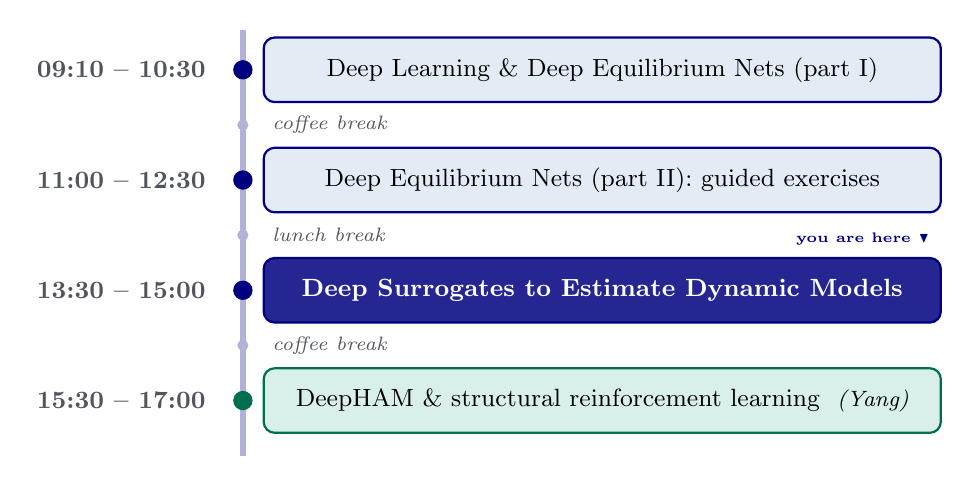
\begin{tikzpicture}[
    session/.style={rectangle, rounded corners=4pt, draw=uzhblue, thick, fill=softblue!15,
                    minimum width=8.6cm, minimum height=0.82cm, align=left, font=\small,
                    inner xsep=10pt, anchor=west},
    now/.style={session, fill=uzhblue!85, draw=uzhblue, text=white, font=\small\bfseries},
    guest/.style={session, fill=softgreen!15, draw=softgreen!70!black},
    pause/.style={font=\scriptsize\itshape, text=uzhgreydark, anchor=west},
    time/.style={font=\small\bfseries, text=uzhgreydark, anchor=east}
]
    \draw[uzhblue!30, line width=2pt] (0,0.5) -- (0,-4.9);

    \node[time] at (-0.35, 0) {09:10 -- 10:30};
    \node[session] at (0.25, 0) {Deep Learning \& Deep Equilibrium Nets (part I)};
    \fill[uzhblue] (0,0) circle (3.5pt);

    \node[pause] at (0.25,-0.7) {coffee break};
    \fill[uzhblue!30] (0,-0.7) circle (2pt);

    \node[time] at (-0.35,-1.4) {11:00 -- 12:30};
    \node[session] at (0.25,-1.4) {Deep Equilibrium Nets (part II): guided exercises};
    \fill[uzhblue] (0,-1.4) circle (3.5pt);

    \node[pause] at (0.25,-2.1) {lunch break};
    \fill[uzhblue!30] (0,-2.1) circle (2pt);

    \node[time] at (-0.35,-2.8) {13:30 -- 15:00};
    \node[now] at (0.25,-2.8) {Deep Surrogates to Estimate Dynamic Models};
    \fill[uzhblue] (0,-2.8) circle (3.5pt);
    \node[font=\tiny\bfseries, text=uzhblue, anchor=south east] at (8.85,-2.35) {you are here $\blacktriangledown$};

    \node[pause] at (0.25,-3.5) {coffee break};
    \fill[uzhblue!30] (0,-3.5) circle (2pt);

    \node[time] at (-0.35,-4.2) {15:30 -- 17:00};
    \node[guest] at (0.25,-4.2) {DeepHAM \& structural reinforcement learning~~{\footnotesize\itshape (Yang)}};
    \fill[softgreen!70!black] (0,-4.2) circle (3.5pt);
\end{tikzpicture}
\end{center}

\vspace{0.1cm}
\begin{center}
{\footnotesize \textbf{Materials:}~\href{https://github.com/sischei/summer-school-AI-for-economics-and-finance-2026}{github.com/sischei/summer-school-AI-\ldots-2026}~~$\cdot$~~\textbf{Cloud:}~\href{https://nuvolos.cloud}{nuvolos.cloud}}
\end{center}
\end{frame}

% --- Slide 3: Roadmap ---
\begin{frame}{Roadmap of This Lecture (90 min)}
\begin{columns}[T]
\column{0.48\textwidth}
\textbf{I.\ What Is a Surrogate?}~~\mbox{\small (12 min)}
\begin{itemize}\setlength\itemsep{1pt}
    \item Look-up tables, pseudo-states, and what the speed-up buys
\end{itemize}

\vspace{0.4em}
\textbf{II.\ Estimate:} structural estimation~~\mbox{\small (20 min)}
\begin{itemize}\setlength\itemsep{1pt}
    \item SMM on a surrogate; Brock--Mirman; the identification ridge
\end{itemize}

\vspace{0.4em}
\textbf{III.\ Gaussian Processes}~~\mbox{\small (24 min)}
\begin{itemize}\setlength\itemsep{1pt}
    \item When data is expensive, a deep net is the wrong tool
    \item Kernels, credible bands, and active learning
\end{itemize}

\column{0.48\textwidth}
\textbf{IV.\ Quantify:} uncertainty~~\mbox{\small (10 min)}
\begin{itemize}\setlength\itemsep{1pt}
    \item Univariate effects, Sobol' indices, Shapley values for the SCC
\end{itemize}

\vspace{0.4em}
\textbf{V.\ Design:} the optimal carbon tax~~\mbox{\small (16 min)}
\begin{itemize}\setlength\itemsep{1pt}
    \item Policy coefficients as pseudo-states; 500 solves, not a million
\end{itemize}

\vspace{0.4em}
\textbf{VI.\ Synthesis and Hands-On}~~\mbox{\small (8 min)}
\begin{itemize}\setlength\itemsep{1pt}
    \item When to use what; the notebooks
\end{itemize}
\end{columns}
\end{frame}

% --- Slide 4: Learning objectives ---
\begin{frame}{Learning Objectives}
\textbf{By the end of this lecture you should be able to:}
\begin{itemize}\itemsep3pt
  \item Explain a surrogate as a \emphc{differentiable look-up table} and say precisely which classical bottleneck it removes
  \item Promote structural or policy parameters to \emphc{pseudo-states}, so that one solve answers a whole family of questions
  \item Estimate a structural parameter by simulated method of moments on a trained surrogate, and read an identification ridge off the criterion surface
  \item Turn the same surrogate into a global sensitivity analysis: univariate effects, Sobol' indices, Shapley values
  \item Fit a Gaussian process, read its credible band, and \emphc{decide between a GP and a deep network} from the cost of one model evaluation
  \item Place the next expensive evaluation where it buys the most, using Bayesian active learning
\end{itemize}
\end{frame}

% ============================================================================
% PART I: WHAT IS A SURROGATE?
% ============================================================================

\section{What Is a Surrogate?}

\begin{frame}{}
\begin{center}
{\Huge \textcolor{uzhblue}{Part I}}\\[0.8em]
{\LARGE What Is a Surrogate?}
\end{center}
\end{frame}

% --- Motivation ---
\begin{frame}{The Bottleneck Is Always the Same}
\begin{block}{Expensive to evaluate}
One evaluation of a modern structural model means solving a Bellman equation, a PDE, or a Monte Carlo simulation: minutes to hours.
\end{block}

\vspace{0.25cm}
\textbf{And we almost never want just one evaluation:}
\begin{itemize}\itemsep2pt
  \item \emphc{Estimation} sweeps thousands of candidate parameter vectors.
  \item \emphc{Uncertainty quantification} propagates a distribution over parameters.
  \item \emphc{Policy design} optimizes over a space of policy rules.
\end{itemize}

\vspace{0.25cm}
\begin{alertblock}{The one advantage we have}
\emphc{We own the model.} Unlike an econometrician with a fixed sample, we can generate as much training data as we are willing to pay for, and the labels are exact.
\end{alertblock}
\end{frame}

% --- Look-up tables -> neural networks ---
\begin{frame}{Look-up Tables $\to$ Neural Networks}
\begin{columns}[T]
\begin{column}{0.40\textwidth}
\textbf{The old idea:} pre-compute once, then interpolate.
\vspace{2pt}
\begin{center}
\footnotesize
\begin{tabular}{cc}
\toprule
$x$ & $\Phi(x)$ \\
\midrule
$-2.0$ & $0.0228$ \\
$-1.0$ & $0.1587$ \\
$\phantom{-}0.0$ & $0.5000$ \\
$\phantom{-}1.0$ & $0.8413$ \\
$\phantom{-}2.0$ & $0.9772$ \\
\bottomrule
\end{tabular}
\end{center}
\vspace{2pt}
{\footnotesize The normal CDF table in the back of every old statistics textbook. Nobody re-derives $\Phi$; they look it up.}
\end{column}

\begin{column}{0.57\textwidth}
\textbf{A 21st-century look-up table:}\\[2pt]
a network that has memorized $\x \mapsto y$,
\[
\surr(\x \,|\, \netw) \;\approx\; y = f(\x).
\]
\vspace{-6pt}
\begin{center}
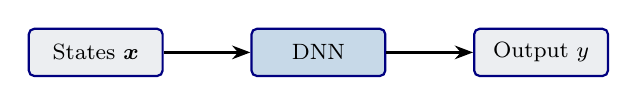
\begin{tikzpicture}[
    mlstep/.style={rectangle, draw=uzhblue, fill=uzhgreylight,
        minimum width=1.7cm, minimum height=0.6cm, font=\footnotesize,
        rounded corners=2pt, thick},
    >=Stealth
]
\node[mlstep] (input) {States $\x$};
\node[mlstep, right=1.1cm of input, fill=softblue!30] (dnn) {DNN};
\node[mlstep, right=1.1cm of dnn] (output) {Output $y$};
\draw[->, thick] (input) -- (dnn);
\draw[->, thick] (dnn) -- (output);
\end{tikzpicture}
\end{center}
\vspace{2pt}
{\footnotesize A table has one entry per grid point and dies of the curse of dimensionality. A network is \emphc{continuous}, \emphc{differentiable}, and its cost grows with the complexity of $f$, not with $n_g^{d}$.}
\end{column}
\end{columns}
\end{frame}

% --- Pseudo-states ---
\begin{frame}{Pseudo-States: The Whole Trick}
\begin{block}{Chen, Didisheim \& Scheidegger (2026)}
Do not build one surrogate per parameter vector. Treat the parameters as \emphc{extra state variables}:
\vspace{-2pt}
\[
\tilde{\x} = \bigl(\underbrace{s_1,\dots,s_n}_{\text{states}},\;
\underbrace{\theta_1,\dots,\theta_p}_{\text{parameters}}\bigr) \in \R^{d},
\qquad d = n + p .
\]
\vspace{-8pt}
\end{block}

\vspace{-0.1cm}
\begin{center}
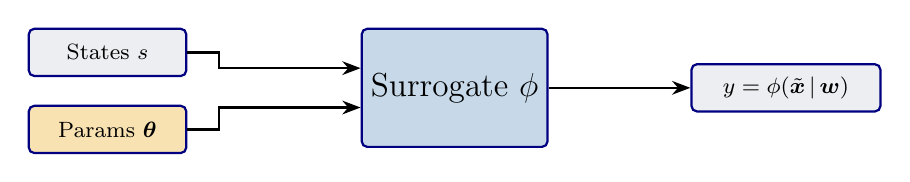
\begin{tikzpicture}[
    mlstep/.style={rectangle, draw=uzhblue, fill=uzhgreylight,
        minimum width=2cm, minimum height=0.6cm, font=\footnotesize,
        rounded corners=2pt, thick},
    >=Stealth
]
\node[mlstep] (states) {States $s$};
\node[mlstep, below=0.35cm of states, fill=softorange!30] (params) {Params $\str$};
\node[mlstep, right=2.2cm of states, yshift=-0.45cm, fill=softblue!30,
      minimum width=2.2cm, minimum height=1.5cm] (surr) {\large Surrogate $\surr$};
\node[mlstep, right=1.8cm of surr, minimum width=2.4cm] (output) {$y = \surr(\tilde{\x}\,|\,\netw)$};
\draw[->, thick] (states.east) -- ++(0.4,0) |- ([yshift=0.25cm]surr.west);
\draw[->, thick] (params.east) -- ++(0.4,0) |- ([yshift=-0.25cm]surr.west);
\draw[->, thick] (surr) -- (output);
\end{tikzpicture}
\end{center}

\vspace{0.1cm}
Solve the model \emphc{once} over the augmented space $\Rightarrow$ an instant answer for \emph{any} parameter configuration in the box. Everything in the rest of this lecture is a different question asked of that one object.
\end{frame}

% --- Building the surrogate ---
\begin{frame}{Building One, in Four Steps}
\small
\begin{enumerate}\itemsep2pt
  \item \textbf{Design.} Draw $\tilde{\x}_i$, $i = 1,\dots,m$, over the box $\prod_j [\underline{x}_j, \bar{x}_j]$: uniform, Latin hypercube, Sobol' sequence, or (Part III) actively.
  \item \textbf{Label.} Evaluate the expensive model: $y_i = f(\tilde{\x}_i)$. \emphc{This is the step that costs money.}
  \item \textbf{Train.} Minimize the empirical risk
  \[
  \hat{\netw} = \argmin_{\netw}\; \frac{1}{m}\sum_{i=1}^{m}
  \bigl|\surr(\tilde{\x}_i\,|\,\netw) - y_i\bigr|^2 .
  \]
  \item \textbf{Validate.} Held-out max and mean absolute error, and for parametric surrogates, error \emph{as a function of} $\str$, not just on average.
\end{enumerate}

\vspace{0.15cm}
\begin{block}{Where the error actually comes from}
Because data is unlimited, scarcity-driven overfitting is not the binding constraint. What binds is \emphc{approximation error} (network capacity against the true regularity of $f$) and \emphc{label noise} when $f$ is itself an approximate inner solver.
\end{block}
\end{frame}

% --- Why surrogates != standard ML ---
\begin{frame}{Not Ordinary Supervised Learning}
\small
\begin{columns}[T]
\begin{column}{0.48\textwidth}
\textbf{Standard supervised learning}
\begin{itemize}\itemsep1pt
  \item Data is scarce and noisy
  \item Overfitting is the main enemy
  \item Regularization, early stopping, cross-validation
  \item Careful tuning, small learning rates
\end{itemize}
\end{column}
\begin{column}{0.48\textwidth}
\textbf{Surrogate modeling}
\begin{itemize}\itemsep1pt
  \item Data is \textbf{unlimited}: we own the model
  \item Labels are \textbf{exact} up to solver tolerance
  \item Large budgets, aggressive learning rates
  \item Focus on \emph{approximation}, not generalization
\end{itemize}
\end{column}
\end{columns}

\vspace{0.3cm}
\begin{block}{What a trained surrogate gives you}
\begin{itemize}\itemsep1pt
  \item \emphc{Accurate enough for the downstream task}: in the option-pricing benchmark, 95th-percentile implied-vol errors below $0.13\%$ of the mean, rising to $0.43\%$ under a week to maturity. \emphc{Accuracy is not uniform over the box}
  \item \textbf{Orders of magnitude faster}, and \textbf{differentiable}: gradients in $\str$ free, by autodiff
\end{itemize}
\end{block}
\end{frame}

% --- Speed comparison ---
\begin{frame}{What the Speed-Up Buys}
\begin{center}
{\footnotesize Table 2 of Chen, Didisheim \& Scheidegger (2026), \emph{Journal of Financial Economics}, for the Bates model:}

\vspace{0.2cm}
\small
\begin{tabular}{l r r r}
\toprule
\textbf{All SPX options on an average day} & \textbf{FFT} & \textbf{Surrogate} & \textbf{$+$ GPU} \\
\midrule
Pricing, 1 day (${\approx}4{,}000$ options) & $10$ s & $0.6$ s & $0.06$ s \\
Gradient, 1 day & $180$ s & $3.2$ s & $0.3$ s \\
Estimation, 1 year (252 days $\times$ 10 iterations) & $125$ h & $2.2$ h & \emphc{$0.2$} h \\
\bottomrule
\end{tabular}
\end{center}

\vspace{0.3cm}
\begin{alertblock}{The point is not the speed but the new question}
At $125$ hours per pass, re-estimating the model every day for a year was not a slow research project; it was \emphc{not a research project at all}. At $0.2$ hours it becomes an option-implied tail-risk measure with a daily time series.
\end{alertblock}
\end{frame}

% --- Notation ---
\begin{frame}{Notation from Here On}
This is an \emph{estimation and policy} lecture, so one symbol changes meaning relative to this morning.

\vspace{0.2cm}
\begin{center}
\small
\begin{tabular}{l l l}
\toprule
\textbf{Symbol} & \textbf{Meaning here} & \textbf{This morning (DEQN deck)} \\
\midrule
$\str$ & \emphc{structural} parameters (e.g.\ $\varrho$, $\beta$) & not used \\
$\pol$ & \emphc{policy} parameters (tax and transfer rules) & not used \\
$\netw$ & network weights & written $\theta$ \\
$\surr(\cdot\,|\,\netw)$ & the surrogate & $\mathcal{N}_\theta$ \\
\bottomrule
\end{tabular}
\end{center}

\vspace{0.25cm}
\begin{alertblock}{Why the swap}
Every paper in this literature writes $\theta$ for the object being estimated; keeping $\theta$ for network weights would make the SMM criterion in Part II unreadable. \emphc{The weights are never the object of interest here}; they are an implementation detail of the look-up table.
\end{alertblock}
\end{frame}

% --- Three questions ---
\begin{frame}{Three Questions, One Surrogate}
\small
The rest of the lecture is the same object, post-processed three different ways.

\vspace{0.4em}
\begin{center}
\footnotesize
\begin{tabular}{>{\raggedright\arraybackslash}p{0.11\textwidth}>{\raggedright\arraybackslash}p{0.24\textwidth}>{\raggedright\arraybackslash}p{0.35\textwidth}>{\raggedright\arraybackslash}p{0.15\textwidth}}
\toprule
\textbf{Operator} & \textbf{Question} & \textbf{Post-processing} & \textbf{Where} \\
\midrule
\emphc{Estimate} & Which parameters fit the data? & $\argmin$ of an SMM criterion over $\str$ & Part II \\[3pt]
\emphc{Quantify} & Which parameter uncertainties matter? & propagate $p(\str)$ through a quantity of interest: univariate effects, Sobol', Shapley & Part IV \\[3pt]
\emphc{Design} & Which policy is best? & constrained $\argmax$ of a welfare objective over $\pol$ & Part V \\
\bottomrule
\end{tabular}
\end{center}

\vspace{0.4em}
The same skeleton throughout: surrogate~1 solves the equilibrium over states \emph{and} pseudo-states; when the quantity of interest is \emph{itself} expensive, a second surrogate maps parameters to it. \emphc{Part II needs only surrogate~1}: its moments are cheap. Parts IV and V need both, and Part III is about what surrogate~2 should be made of.
\end{frame}

% ============================================================================
% PART II: STRUCTURAL ESTIMATION
% ============================================================================

\section{Estimate: Structural Estimation}

\begin{frame}{}
\begin{center}
{\Huge \textcolor{uzhblue}{Part II}}\\[0.8em]
{\LARGE Estimate: Structural Estimation}
\end{center}
\end{frame}

% --- The estimation loop ---
\begin{frame}{The Estimation Loop, and Why It Is Expensive}
\textbf{The classical nested fixed point.} For each candidate $\str$:
\begin{center}
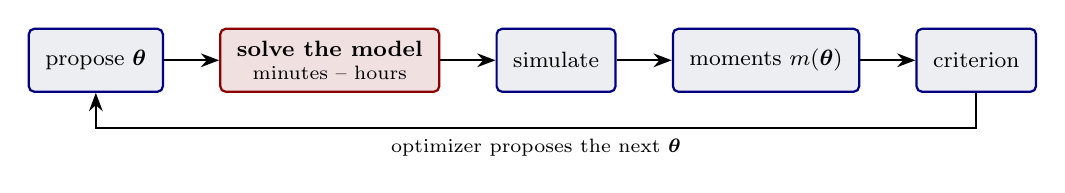
\begin{tikzpicture}[
    box/.style={rectangle, draw=uzhblue, thick, rounded corners=2pt, fill=uzhgreylight,
                minimum height=0.8cm, font=\footnotesize, align=center, inner xsep=6pt},
    >=Stealth
]
\node[box] (guess) {propose $\str$};
\node[box, right=0.7cm of guess, fill=darkred!12, draw=darkred] (solve) {\textbf{solve the model}\\[-1pt]{\scriptsize minutes -- hours}};
\node[box, right=0.7cm of solve] (sim) {simulate};
\node[box, right=0.7cm of sim] (mom) {moments $m(\str)$};
\node[box, right=0.7cm of mom] (crit) {criterion};
\draw[->, thick] (guess) -- (solve);
\draw[->, thick] (solve) -- (sim);
\draw[->, thick] (sim) -- (mom);
\draw[->, thick] (mom) -- (crit);
\draw[->, thick] (crit.south) -- ++(0,-0.45) -| node[pos=0.25, below, font=\scriptsize] {optimizer proposes the next $\str$} (guess.south);
\end{tikzpicture}
\end{center}

\vspace{0.5cm}
\textbf{The surrogate move.} Put $\str$ \emph{inside} the network at training time. The red box then runs \emphc{once}, and the loop becomes a forward pass.

\vspace{0.3cm}
\begin{block}{Two consequences, not one}
\begin{itemize}\itemsep1pt
  \item The criterion becomes cheap enough to evaluate on a fine grid, so you can \emph{look at} it rather than trust a local optimizer's report.
  \item The criterion becomes \emphc{differentiable in $\str$}, because the surrogate is.
\end{itemize}
\end{block}
\end{frame}

% --- SMM 1 ---
\begin{frame}{SMM: The Moment Condition}
\small
Let the data give $T$ observations $\{y_t\}$. Choose moment functions $g(y)\in\R^{q}$ such that, at the true parameter $\str_0 \in \R^{p}$ with $q \ge p$,
\[
\E{g(y_t) - m(\str_0)} = 0,
\qquad m(\str) = \mathbb{E}_{\str}[g(y_t)] .
\]
The empirical and simulated counterparts are
\[
\widehat g_T = \tfrac{1}{T}\sum_{t=1}^{T} g(y_t),
\qquad
\widehat m_S(\str) = \tfrac{1}{S}\sum_{s=1}^{S} g\bigl(y^{\mathrm{sim}}_s(\str)\bigr).
\]

\vspace{0.2em}
\textbf{Identification.} $\str_0$ is the \emph{unique} zero of $\E{g(y_t)} - m(\str)$ on the parameter space. Just-identified: $q = p$. Over-identified: $q > p$, which buys a testable restriction. It does \emph{not} automatically sharpen the criterion: a moment with a near-zero column in $M$ adds noise and finite-sample bias, as the joint exercise will show.

\vspace{0.2em}
\textbf{In this lecture.} $y_t$ is log output, consumption, and capital; $g$ collects three volatility and autocorrelation moments; $\str = \varrho$ first, then $\str = (\beta,\varrho)$.
\end{frame}

% --- SMM 2 ---
\begin{frame}{SMM: Estimator and Weighting}
\small
\[
\widehat{\str}_{\mathrm{SMM}} = \argmin_{\str}\;
\bigl[\widehat g_T - \widehat m_S(\str)\bigr]^{\!\top} W \bigl[\widehat g_T - \widehat m_S(\str)\bigr],
\qquad W \succ 0 .
\]

\vspace{0.3em}
\begin{alertblock}{Common random numbers: the detail that decides success}
Hold the shock draws $\{\varepsilon_s\}$ \emphc{fixed across $\str$}. Then $\widehat m_S(\str)$ is a smooth function of $\str$, with a clean minimum. Re-draw them and you are optimizing a noisy surface: the optimizer chases simulation noise and reports wherever it happened to land.
\end{alertblock}

\vspace{0.2em}
\textbf{Weighting matrix.}
\begin{itemize}\itemsep1pt
  \item \emphc{Identity} $W = I$: the honest pedagogical default; consistent, inefficient.
  \item \emphc{Diagonal} $W = \mathrm{diag}(1/\hat\sigma_g^2)$: rescales each moment by its sampling variance.
  \item \emphc{Optimal} $W^\star = \Omega^{-1}$, the inverse asymptotic covariance of the moment gap, proportional to $\widehat\Sigma_g^{-1}$ up to the simulation factor $1 + 1/S$. Minimum asymptotic variance. ($S = 10$ costs 5\% in standard errors; $S = 1$ costs 41\%.)
\end{itemize}
\end{frame}

% --- SMM 3 ---
\begin{frame}{SMM: What the Asymptotics Tell You to Look At}
\small
Write $M = \partial m(\str_0)/\partial\str^\top$ for the moment Jacobian, and $\Omega$ for the asymptotic covariance of the \emphc{moment gap} $\sqrt{T}\bigl[\widehat g_T - \widehat m_S(\str_0)\bigr]$. If the simulated shocks are drawn independently of the data, $\Omega = (1 + 1/S)\,\widehat\Sigma_g$ with $S$ panels of the data's length; as $S \to \infty$, $\Omega \to \widehat\Sigma_g$. \emphc{The inflation is the price of simulating rather than solving.}

\vspace{0.2em}
Under the usual regularity conditions, as $T \to \infty$,
\[
\sqrt{T}\,\bigl(\widehat{\str}_{\mathrm{SMM}} - \str_0\bigr) \;\xrightarrow{d}\; \mathcal{N}\bigl(0, V(W)\bigr),
\qquad
V(W) = (M^\top W M)^{-1} M^\top W \,\Omega\, W M (M^\top W M)^{-1},
\]
which collapses to $V(W^\star) = (M^\top \Omega^{-1} M)^{-1}$ at the efficient weighting.

\vspace{0.3em}
\begin{block}{Identification, read geometrically}
$V$ exists only if $M$ has \emphc{full column rank}. A near-rank-deficient $M$ is a \emphc{flat direction} of the criterion: an \emph{identification ridge}. Standard errors explode, the point estimate is arbitrary along the ridge, and no amount of data at those moments fixes it.

\vspace{2pt}
Because the surrogate makes the criterion cheap, you can \emphc{plot the ridge} instead of inferring it from an ill-conditioned Hessian. We do exactly that at the end of this part.
\end{block}
\end{frame}

% --- What the surrogate costs you, econometrically ---
\begin{frame}{The Surrogate Is Not Free}
\small
Everything on the previous slide assumed the moments came from \emph{the model}. They came from a network. Write $\widehat m = m + e$, where $e$ is the surrogate's approximation error.

\vspace{0.15cm}
\begin{alertblock}{$e$ does not shrink with the sample}
More data makes $\widehat g_T$ precise; it does nothing to $e$. This is \emphc{non-local misspecification}: the estimator converges not to $\str_0$ but to a \emphc{pseudo-true} $\str^\star$ minimizing the population criterion under $\widehat m$, with Hall--Inoue asymptotics rather than Hansen's.
\vspace{2pt}
\[
\sqrt{T}\bigl(\widehat{\str} - \emphc{\str^\star}\bigr) \;\xrightarrow{d}\; \mathcal{N}\bigl(0, \Sigma(\mu^\star)\bigr),
\qquad \str^\star \to \str_0 \ \text{ only as } \ \sup_{\str} \|e(\cdot,\str)\| \to 0 .
\]
\end{alertblock}

\vspace{0.1cm}
\textbf{The practical consequence}, and the whole reason Part I ended with a validation step: report the surrogate's \emphc{maximum} error over the parameter box, not its mean. The maximum bounds the bias, and a surrogate with excellent \emph{average} accuracy can still be badly wrong in the one direction you are estimating. That happens at the end of this part.

\vspace{0.05cm}
{\footnotesize Chen, Didisheim \& Scheidegger (2026), fn.\ 15, make the point about their own surrogate; the asymptotics are Hall \& Inoue (2003).}
\end{frame}

% --- The model ---
\begin{frame}{The Model: Brock--Mirman with Stochastic TFP}
\small
The same model class as this morning, with two deliberate changes: $\delta$ drops from $1$ to $0.10$, which destroys the closed form, and $\varrho$ is promoted from a fixed number to an input.
\begin{gather*}
\max_{\{C_t\}} \sum_{t=0}^{\infty} \beta^t\, \E{\ln C_t},
\qquad K_{t+1} + C_t = Y_t + (1-\delta)K_t ,\\[4pt]
Y_t = z_t K_t^{\alpha}, \qquad
\log z_{t+1} = \varrho \log z_t + \sigma\,\varepsilon_{t+1},
\qquad \varepsilon_{t+1} \sim \mathcal{N}(0,1).
\end{gather*}

\vspace{0.15cm}
\textbf{Calibration}
\begin{center}\small
\begin{tabular}{cccc}
\toprule
$\alpha$ & $\delta$ & $\sigma$ & $\beta$ (scalar exercise) \\
\midrule
$0.36$ & $0.10$ & $0.04$ & $0.96$ \\
\bottomrule
\end{tabular}
\end{center}

\vspace{0.1cm}
{\footnotesize \emphc{Note the $\delta$.} The textbook closed form $s^\star = \alpha\beta$ needs $\delta = 1$. Here $\delta = 0.10$, so there is \emph{no} analytic policy and the Euler equation must be solved numerically, which is precisely the expensive inner solve the surrogate replaces. Choosing $\delta=1$ would have made the exercise vacuous.}
\end{frame}

% --- Why rho ---
\begin{frame}{Why $\varrho$, and Not $\beta$?}
\small
\begin{itemize}\itemsep3pt
  \item $\beta$ is famously \emphc{poorly identified from business-cycle moments}: volatilities and autocorrelations barely move with it. It does shift the \emph{level} of the capital stock, which is the channel we exploit at the end of this part.
  \item In practice $\beta$ is \emph{calibrated} to a target steady-state interest rate. Under log utility with general $\delta$, the steady-state Euler relation is $1/\beta = 1 + \alpha (k^\star)^{\alpha-1} - \delta$.
  \item $\varrho$ has a \emphc{clean, direct mapping} into autocorrelation moments: $\mathrm{Corr}(\log Y_t, \log Y_{t-1})$ and $\mathrm{Corr}(\Delta \log C_t, \Delta \log C_{t-1})$ both move monotonically with persistence.
  \item So $\varrho$ is the textbook \emphc{sharply identified} scalar, what you want when learning the workflow. Three moments for one parameter is over-identified, which buys a testable restriction; it does \emph{not} automatically sharpen anything.
\end{itemize}

\vspace{0.2cm}
Notebook \texttt{03\_03} does the scalar case. Notebook \texttt{03\_04} then frees $\beta$ as well, and the pathology shows up immediately.
\end{frame}

% --- Step 1 ---
\begin{frame}{Step 1: Train the Surrogate with $\varrho$ as a Pseudo-State}
\small
\begin{block}{Goal}
Learn $\surr:(z_t, K_t, \varrho) \mapsto s_t \in (0,1)$, with $K_{t+1} = (1-\delta)K_t + s_t Y_t$.
\end{block}

\begin{enumerate}\itemsep2pt
  \item A three-input MLP with a \emph{sigmoid} output head, so $s_t \in (0,1)$ holds by construction: the hard-constraint trick from this morning.
  \item Train on the Euler residual with Gauss--Hermite quadrature. \emphc{$\varrho$ enters both the policy and the transition.} Under log utility the notebooks minimize the scale-free \emph{relative} residual, which shares its zero set with the raw one but conditions far better in FP32:
  {\footnotesize\[
  \ell = \frac{1}{N}\sum_i \left(
  \left[\, \beta\, C^{(i)}_t \sum_j w_j \frac{1 - \delta + \alpha z^{(i)}_{t+1,j} K^{(i)\,\alpha-1}_{t+1}}{C^{(i)}_{t+1,j}} \,\right]^{-1} \!\!- 1 \right)^{\!2}
  \]}
  \vspace{-10pt}
  \item Two phases: uniform sampling over the $(z, K, \varrho)$ box, then simulation-based refinement.
  \item Validate by plotting $s(z\!=\!1, K, \varrho)$ across $\varrho$, and ask first how much the policy \emph{should} move with $\varrho$. Here the honest answer is ``not much'', which is worth knowing \emph{before} you diagnose lazy learning.
\end{enumerate}
\end{frame}

% --- Step 2 ---
\begin{frame}{Step 2: Simulate, and Choose Moments That Identify}
\begin{block}{Goal}
Generate synthetic data at $\varrho_{\mathrm{true}} = 0.90$; three identifying moments, plus a counterexample.
\end{block}

\begin{center}\footnotesize
\begin{tabular}{cl}
\toprule
\textbf{Moment} & \textbf{What it captures} \\
\midrule
$m_1 = \mathrm{Std}(\Delta \log C_t)$ & growth-rate volatility \\
$m_2 = \mathrm{Corr}(\Delta \log C_t, \Delta \log C_{t-1})$ & persistence in consumption growth \\
$m_3 = \mathrm{Corr}(\log Y_t, \log Y_{t-1})$ & persistence in output, the most direct \\
\midrule
$m_0 = \mathrm{mean}(s_t)$ \emph{(diagnostic)} & \emphc{nearly flat in $\varrho$, what not to use here} \\
\bottomrule
\end{tabular}\end{center}

\vspace{0.1cm}
{\footnotesize \textbf{A trap:} $\mathrm{Var}(\log z) = \sigma^2/(1-\varrho^2)$ increases in $\varrho$, but $\mathrm{Var}(\Delta\log z) = 2\sigma^2/(1+\varrho)$ \emph{decreases}.

\vspace{2pt}
\textbf{And be clear what the ``data'' are:} one simulation of the surrogate itself at $\varrho = 0.90$, under the \emph{same} shock path as every candidate. Deliberate: it isolates identification from sampling noise, but the criterion then hits exactly zero. \emphc{This validates the machinery, not the estimator's finite-sample behavior.}}
\end{frame}

% --- Step 3 ---
\begin{frame}{Step 3: Minimize the Criterion}
\small
\begin{block}{The scalar case, $\str = \varrho$}
\vspace{-6pt}
\[\hat\varrho = \argmin_{\varrho}\; [m(\varrho) - \hat m^{\mathrm{data}}]^\top W\, [m(\varrho) - \hat m^{\mathrm{data}}], \qquad W = I .\]
\vspace{-8pt}
\end{block}

\begin{enumerate}\itemsep2pt
  \item One routine $\varrho \mapsto (C_t, I_t, Y_t) \mapsto m(\varrho)$, reusing the trained surrogate throughout.
  \item Evaluate on a fine grid over $[0.50, 0.99]$, step $0.005$, 99 points. \emphc{At surrogate speed this is cheaper than one call to the original model.}
  \item Take the grid $\argmin$. No separate optimizer is needed, and you see the whole criterion rather than one path through it.
  \item \emphc{Check the solution is interior.} A corner solution invalidates the asymptotics we just set up, and usually signals a mis-specified moment.
\end{enumerate}

\vspace{0.15cm}
{\footnotesize $W = I$ is inefficient but consistent; the efficient $W^\star = \widehat\Sigma_g^{-1}$ changes the standard errors, not the argument.}
\end{frame}

% --- Result 1 ---
\begin{frame}{Result: The Surrogate Slice $s(K, \varrho \mid z = 1)$}
\begin{center}
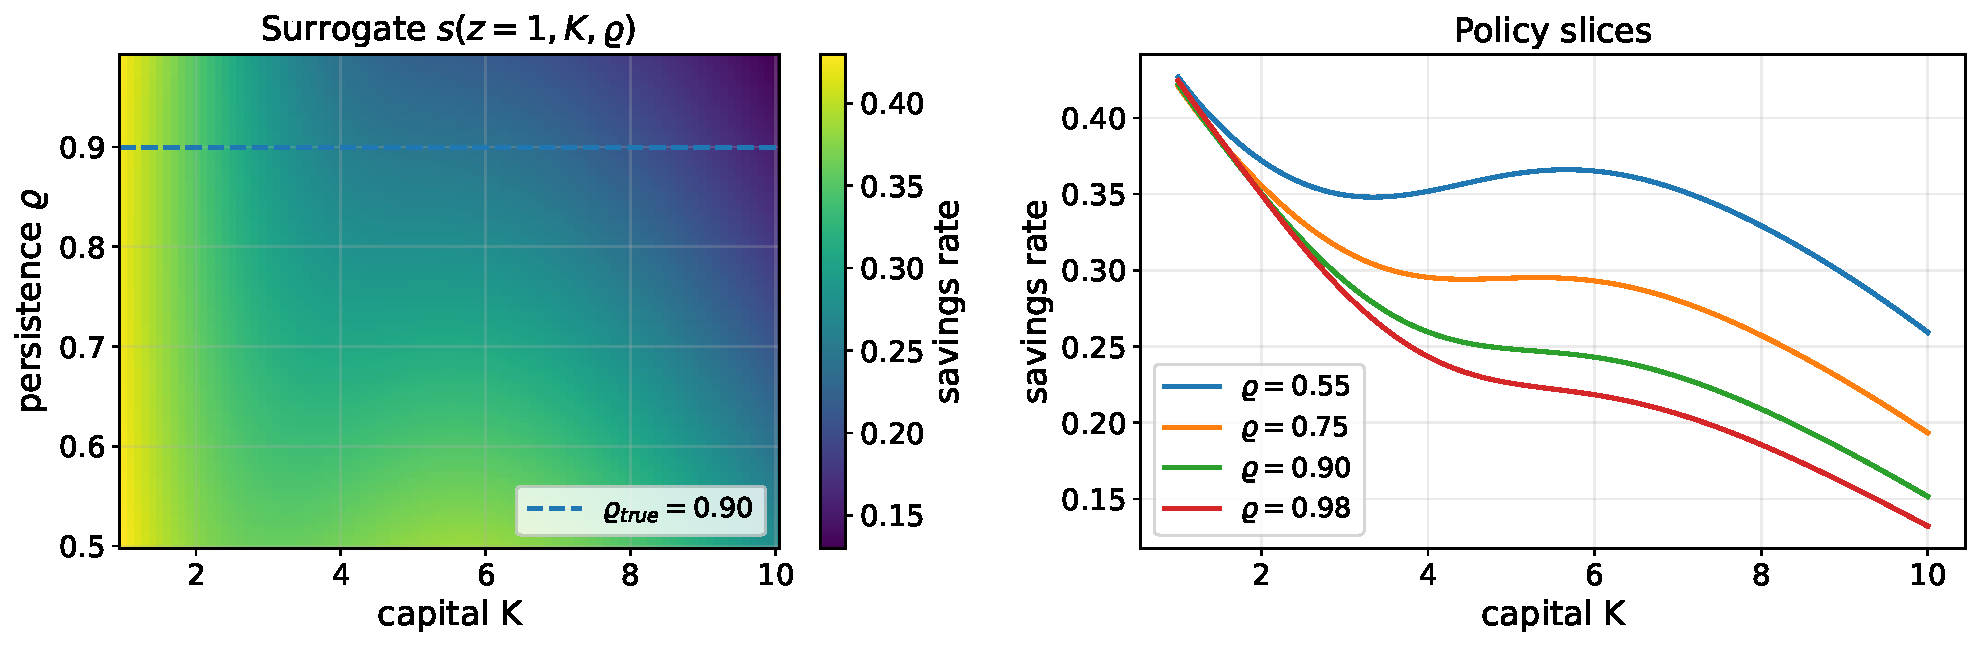
\includegraphics[width=0.94\textwidth]{figures/rho_surrogate_heatmap.pdf}
\end{center}
\vspace{-0.1cm}
{\footnotesize One trained object standing in for 99 separate model solutions. Note what it does \emph{not} show: the policy depends strongly on $K$ and only \emphc{weakly} on $\varrho$: the four slices differ by only a few per cent at low $K$, and $\varrho = 0.90$ and $0.98$ nearly coincide. That is not a defect. Most of the identifying information sits in the \emph{transition}, not the policy: $\varrho$ sets the persistence of $z$, and the moments are autocorrelations of simulated paths.}
\end{frame}

% --- Result 2 ---
\begin{frame}{Result: Which Moments Actually Identify}
\begin{center}
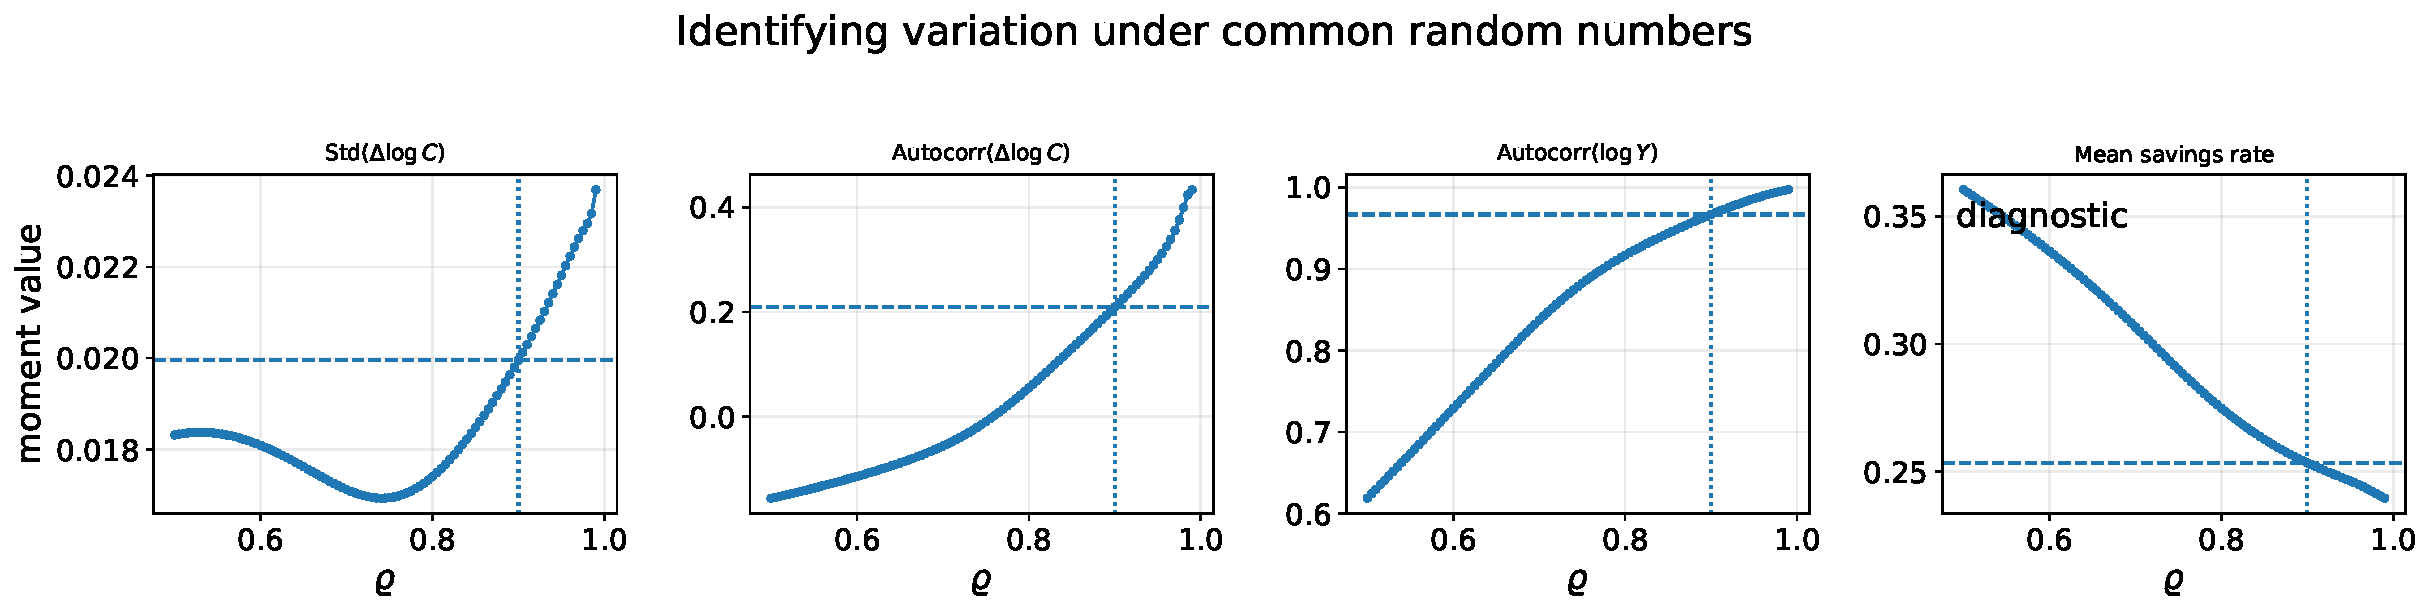
\includegraphics[width=0.96\textwidth]{figures/rho_identification.pdf}
\end{center}
\vspace{-0.1cm}
{\footnotesize $m_2$ and $m_3$ rise monotonically in $\varrho$: either alone would pin the parameter down. $m_1$ is \emphc{U-shaped}: nearly flat below $\varrho \approx 0.75$, steep above it, so it identifies well near the truth and barely at all in the lower half of the range. The diagnostic $m_0$ is \emphc{essentially flat}: its measured slope at $\varrho_{\mathrm{true}}$ is $-0.07$, against $+1.02$ for $m_2$. A moment with no slope contributes a near-zero column to $M$, and therefore almost nothing to identification, however well it matches in the data.}
\end{frame}

% --- Result 3 ---
\begin{frame}{Result: The Criterion and the Estimate}
\begin{center}
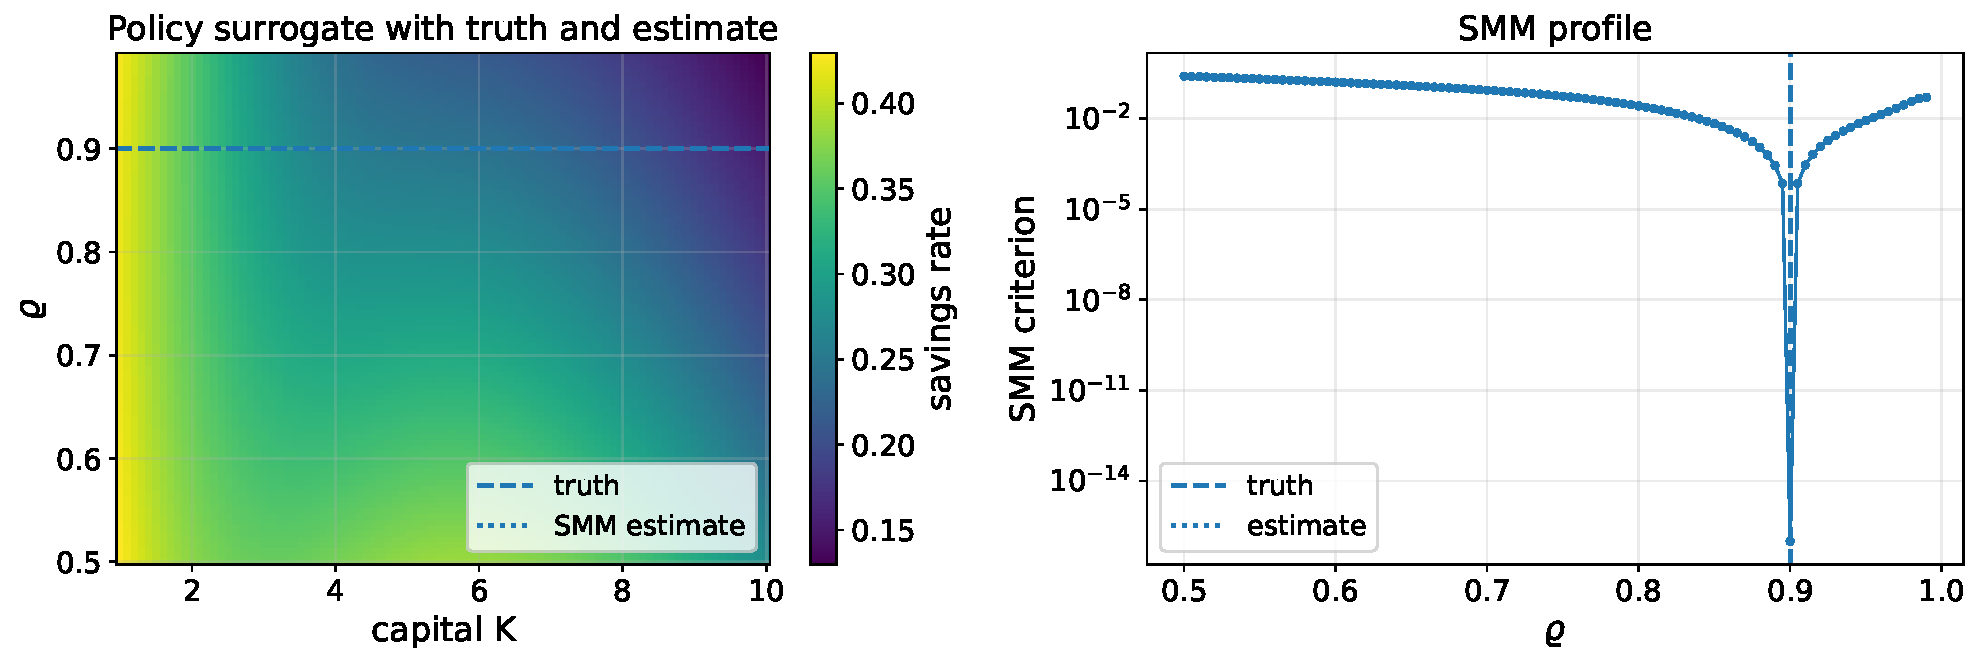
\includegraphics[width=0.94\textwidth]{figures/rho_estimate_on_surrogate.pdf}
\end{center}
\vspace{-0.1cm}
{\footnotesize A single sharp interior minimum at $\hat\varrho = \emphc{0.900}$, exact because of the design on the previous slide, not because of luck. Note the \emph{log} vertical axis: the criterion falls by three orders of magnitude between $\varrho = 0.8$ and the minimum. \emphc{Curvature this steep is what good identification looks like}, but with a zero-noise design we cannot turn it into a standard error. Contrast the next slide.}
\end{frame}

% --- Joint estimation: the ridge, and how it closes ---
\begin{frame}{Joint Estimation of $(\beta,\varrho)$: A Ridge, and How It Closes}
\begin{center}
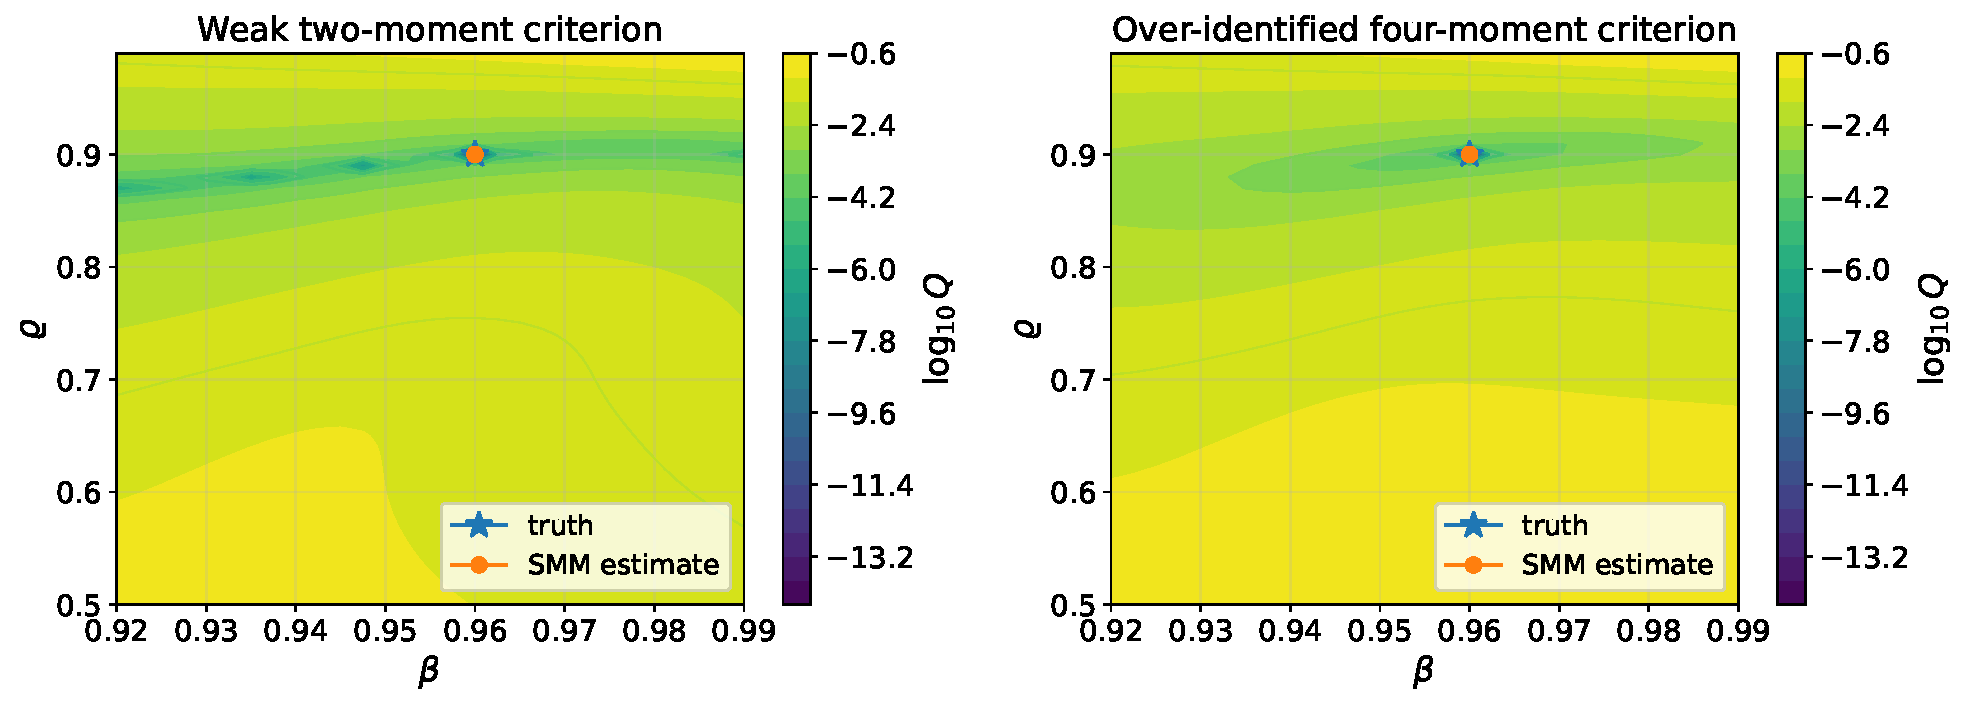
\includegraphics[width=0.94\textwidth]{figures/joint_criterion_contour.pdf}
\end{center}

\vspace{-0.25cm}
\footnotesize
\begin{columns}[T]
\column{0.48\textwidth}
\textbf{Two dynamic moments.} A long valley along $\beta$: many $(\beta,\varrho)$ pairs fit about equally well.
\emphc{Condition number 96}, smallest singular value $0.021$.
\column{0.48\textwidth}
\textbf{Add the level moments.} The valley closes into a basin.
\emphc{Condition number 2.5}, smallest singular value $0.91$.
\end{columns}

\vspace{0.15cm}
{\footnotesize The classical result: $\beta$ moves the capital stock's \emph{level}, so a level moment identifies it and business-cycle moments do not. \emphc{Identification is fixed by information, not by a better optimizer.}}
\end{frame}

% --- The ridge that wasn't ---
\begin{frame}{The Ridge That Wasn't}
\small
An earlier run of this same notebook produced a ridge that \textbf{stayed open} when the level moments were added: condition number $305$, the weak direction lying almost exactly along the $\beta$ axis. It looked like a clean econometric finding. It was not.

\vspace{0.15cm}
\begin{columns}[T]
\column{0.5\textwidth}
\begin{center}
\footnotesize
\begin{tabular}{lrr}
\toprule
& \textbf{200 steps} & \textbf{8{,}000 steps} \\
\midrule
$s$ at the anchor & $0.336$ & $0.254$ \\
error vs.\ $s^\star = 0.254$ & \emphc{$32\%$} & $0.0\%$ \\
$\partial m_0 / \partial \beta$ & \emphc{$-0.0016$} & $+1.27$ \\
condition number & $305$ & $2.5$ \\
\bottomrule
\end{tabular}
\end{center}
\column{0.46\textwidth}
The closed form gives $\mathrm{d}s^\star/\mathrm{d}\beta = 1.92$. The under-trained surrogate reported $-0.0016$: \emphc{near zero and the wrong sign}. Its Euler loss looked fine.
\end{columns}

\vspace{0.12cm}
\begin{alertblock}{The check that catches it}
A flat direction is either the moments or \emphc{the surrogate}, and the criterion cannot tell you which. Evaluate the surrogate against something known in closed form first: here $s^\star(\beta)$ at the steady state. This is \emph{lazy learning} from this morning's Part VI, caught in the act.
\end{alertblock}
\end{frame}

% --- Production ---
\begin{frame}{From Classroom to Production}
\small
Brock--Mirman is the mechanism in miniature. Chen, Didisheim \& Scheidegger (2026) run it on a high-dimensional workhorse option-pricing model.

\vspace{0.2cm}
\begin{columns}[T]
\column{0.48\textwidth}
\textbf{What the surrogate enables}
\begin{itemize}\itemsep1pt
  \item Re-estimate \emphc{every day} instead of once per paper
  \item Systematic out-of-sample evaluation against reduced-form benchmarks
  \item Conditional distributions of option returns
\end{itemize}

\column{0.48\textwidth}
\textbf{What that produced}
\begin{itemize}\itemsep1pt
  \item An option-implied \emphc{tail-risk index}, predictive of market crashes
  \item A \emphc{parameter-instability} measure that lines up with option-market illiquidity
  \item A read on the structural-versus-reduced-form trade-off
\end{itemize}
\end{columns}

\vspace{0.25cm}
\begin{alertblock}{The pattern worth remembering}
None of these are faster versions of old results. They are questions whose \emph{answers require a time series of estimates}, and that is exactly what a parametric surrogate manufactures.
\end{alertblock}
\end{frame}

% ============================================================================
% PART III: GAUSSIAN PROCESSES
% ============================================================================

\section{Gaussian Processes}

\begin{frame}{}
\begin{center}
{\Huge \textcolor{uzhblue}{Part III}}\\[0.8em]
{\LARGE Gaussian Processes:\\[0.3em] When Data Is Expensive}
\end{center}
\end{frame}

% --- Why GPs ---
\begin{frame}{When One Label Costs Four Hours}
\small
\textbf{Everything so far assumed labels are cheap.} For option pricing they are: $10^6$ evaluations is an afternoon. \emphc{That fails the moment the model is a global stochastic equilibrium.}

\vspace{0.15cm}
\begin{columns}[T]
\column{0.48\textwidth}
\textbf{What a deep network needs}
\begin{itemize}\itemsep1pt
  \item $10^4$ to $10^6$ labeled points
  \item An architecture and hyperparameters to search for
  \item Many epochs of SGD, and no uncertainty unless you train an ensemble
\end{itemize}

\column{0.48\textwidth}
\textbf{What a Gaussian process needs}
\begin{itemize}\itemsep1pt
  \item Tens to a few thousand points
  \item A kernel: an explicit smoothness assumption
  \item A closed-form posterior, no SGD, and \emphc{posterior variance everywhere, for free}
\end{itemize}
\end{columns}

\vspace{0.2cm}
\begin{alertblock}{Why the variance is the real prize}
It is not decoration: it tells you \emphc{where the surrogate does not know the answer}. That is what lets you spend the next expensive evaluation well, and what says whether a welfare surface is trustworthy before you optimize it.
\end{alertblock}
\end{frame}

% --- Multivariate Gaussians ---
\begin{frame}{Recall: Multivariate Gaussians}
\begin{columns}[T]
\column{0.45\textwidth}
A random vector $\x \in \R^d$ is multivariate Gaussian if
\[
\x \sim \mathcal{N}(\bm{\mu}, \Sigma),
\]
with density
{\small
\[
p(\x) \propto \exp\!\Bigl(-\tfrac{1}{2}(\x - \bm{\mu})^\top \Sigma^{-1} (\x - \bm{\mu})\Bigr).
\]
}

\vspace{0.2cm}
\begin{block}{Key fact}
It is \emphc{fully characterized} by $\bm{\mu}$ and $\Sigma$. Nothing else about the distribution is free.
\end{block}
\column{0.52\textwidth}
\begin{center}
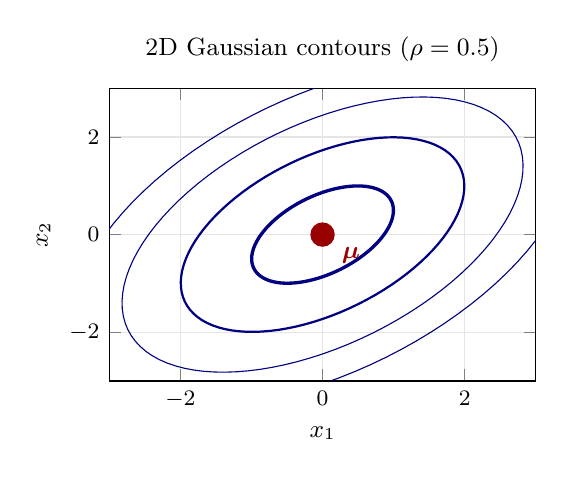
\begin{tikzpicture}
\begin{axis}[
    width=7cm, height=5.3cm,
    xlabel={$x_1$}, ylabel={$x_2$},
    xmin=-3, xmax=3, ymin=-3, ymax=3,
    grid=major, grid style={gray!20},
    every axis plot/.append style={no markers},
    title={2D Gaussian contours ($\rho = 0.5$)},
]
\addplot[uzhblue, very thick, domain=0:360, samples=100]
    ({0.707*(1.22*cos(x) - 0.707*sin(x))}, {0.707*(1.22*cos(x) + 0.707*sin(x))});
\addplot[uzhblue, thick, domain=0:360, samples=100]
    ({1.414*(1.22*cos(x) - 0.707*sin(x))}, {1.414*(1.22*cos(x) + 0.707*sin(x))});
\addplot[uzhblue, domain=0:360, samples=100]
    ({2.0*(1.22*cos(x) - 0.707*sin(x))}, {2.0*(1.22*cos(x) + 0.707*sin(x))});
\addplot[uzhblue, thin, domain=0:360, samples=100]
    ({2.5*(1.22*cos(x) - 0.707*sin(x))}, {2.5*(1.22*cos(x) + 0.707*sin(x))});
\addplot[only marks, mark=+, mark size=4pt, harvardcrimson, thick] coordinates {(0,0)};
\node[font=\small, harvardcrimson] at (axis cs:0.4,-0.42) {$\bm{\mu}$};
\end{axis}
\end{tikzpicture}
\end{center}
\end{columns}
\end{frame}

% --- Conditioning is regression ---
\begin{frame}{Conditioning Is Regression}
\begin{columns}[T]
\column{0.48\textwidth}
\textbf{Joint:}
\[
\begin{pmatrix} x_1 \\ x_2 \end{pmatrix} \sim
\mathcal{N}\!\left(
\begin{pmatrix} \mu_1 \\ \mu_2 \end{pmatrix},
\begin{pmatrix} \Sigma_{11} & \Sigma_{12} \\ \Sigma_{21} & \Sigma_{22}\end{pmatrix}
\right)
\]

\vspace{0.25cm}
\textbf{Conditional:}
\begin{align*}
\mu_{1|2} &= \mu_1 + \Sigma_{12}\Sigma_{22}^{-1}(x_2 - \mu_2)\\
\Sigma_{1|2} &= \Sigma_{11} - \Sigma_{12}\Sigma_{22}^{-1}\Sigma_{21}
\end{align*}

\vspace{0.15cm}
\emphc{These two lines are the entire engine of GP regression.} Everything that follows is bookkeeping about how to build $\Sigma$.

\column{0.50\textwidth}
\begin{center}
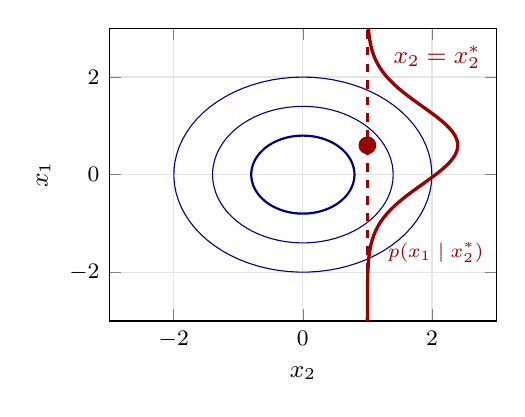
\begin{tikzpicture}
\begin{axis}[
    width=6.5cm, height=5.3cm,
    xlabel={$x_2$}, ylabel={$x_1$},
    xmin=-3, xmax=3, ymin=-3, ymax=3,
    grid=major, grid style={gray!20},
    every axis plot/.append style={no markers},
]
\addplot[uzhblue, thick, domain=0:360, samples=80]
    ({0.8*(0.894*cos(x) - 0.447*sin(x))}, {0.8*(0.447*cos(x) + 0.894*sin(x))});
\addplot[uzhblue, domain=0:360, samples=80]
    ({1.4*(0.894*cos(x) - 0.447*sin(x))}, {1.4*(0.447*cos(x) + 0.894*sin(x))});
\addplot[uzhblue, thin, domain=0:360, samples=80]
    ({2.0*(0.894*cos(x) - 0.447*sin(x))}, {2.0*(0.447*cos(x) + 0.894*sin(x))});
\draw[harvardcrimson, very thick, dashed] (axis cs:1,-3) -- (axis cs:1,3);
\node[font=\small, harvardcrimson, anchor=north east] at (axis cs:2.9,2.85) {$x_2 = x_2^*$};
\addplot[harvardcrimson, very thick, domain=-3:3, samples=80]
    ({1 + 1.4*exp(-(x-0.6)^2/(2*0.64))}, {x});
\node[font=\scriptsize, harvardcrimson, anchor=east, inner sep=1pt] at (axis cs:2.85,-1.6) {$p(x_1 \mid x_2^*)$};
\addplot[only marks, mark=*, mark size=3pt, harvardcrimson] coordinates {(1,0.6)};
\end{axis}
\end{tikzpicture}
\end{center}
{\small Slicing the joint at $x_2 = x_2^*$ leaves a 1D Gaussian: a prediction \emph{and} an error bar.}
\end{columns}
\end{frame}

% --- From observations to interpolation ---
\begin{frame}{From Observations to Interpolation}
\vspace{-0.2cm}
\begin{columns}[T]
\column{0.36\textwidth}
\begin{center}
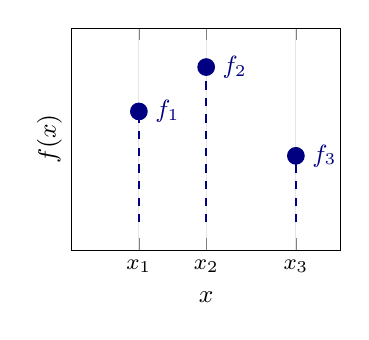
\begin{tikzpicture}
\begin{axis}[
    width=5.0cm, height=4.4cm,
    xlabel={$x$}, ylabel={$f(x)$},
    xmin=-0.5, xmax=5.5, ymin=-0.5, ymax=3.5,
    grid=major, grid style={gray!20},
    xtick={1,2.5,4.5}, xticklabels={$x_1$,$x_2$,$x_3$},
    ytick=\empty,
    every axis plot/.append style={no markers},
]
\addplot[uzhblue, thick, dashed] coordinates {(1,0) (1,2.0)};
\addplot[uzhblue, thick, dashed] coordinates {(2.5,0) (2.5,2.8)};
\addplot[uzhblue, thick, dashed] coordinates {(4.5,0) (4.5,1.2)};
\addplot[only marks, mark=*, mark size=3pt, uzhblue] coordinates {(1,2.0) (2.5,2.8) (4.5,1.2)};
\node[font=\small, uzhblue, anchor=west] at (axis cs:1.15,2.0) {$f_1$};
\node[font=\small, uzhblue, anchor=west] at (axis cs:2.65,2.8) {$f_2$};
\node[font=\small, uzhblue, anchor=west] at (axis cs:4.65,1.2) {$f_3$};
\end{axis}
\end{tikzpicture}
\end{center}
\column{0.58\textwidth}
\textbf{Assume} the function values are jointly Gaussian:
\vspace{-0.2cm}
{\small
\[
\begin{pmatrix} f_1 \\ f_2 \\ f_3 \end{pmatrix} \sim
\mathcal{N}\!\left(\bm{0},\;
\begin{pmatrix} K_{11} & K_{12} & K_{13} \\ K_{21} & K_{22} & K_{23} \\ K_{31} & K_{32} & K_{33}\end{pmatrix}\right)
\]
}

\vspace{-0.1cm}
\emphc{Nearby points should be more correlated than distant ones.} With a squared-exponential kernel and $\ell = 2$:
\[
K = \begin{pmatrix} 1.00 & 0.76 & 0.22 \\ 0.76 & 1.00 & 0.61 \\ 0.22 & 0.61 & 1.00 \end{pmatrix}
\]

\vspace{0.1cm}
Build the covariance from a \emphc{kernel}, $K_{ij} = k(x_i,x_j)$. Conditioning on the observed $f_i$ then predicts everywhere else.
\end{columns}
\end{frame}

% --- GP definition ---
\begin{frame}{A Gaussian Process: A Distribution over Functions}
\begin{block}{Definition}
A \emphc{Gaussian process} is a collection of random variables, any finite subset of which is jointly Gaussian:
\[
f(\x) \sim \mathcal{GP}\bigl(\mu(\x),\; k(\x,\x')\bigr).
\]
\end{block}

\begin{itemize}\itemsep2pt
  \item \textbf{Mean function} $\mu(\x) = \E{f(\x)}$, almost always $0$ after centering the data.
  \item \textbf{Covariance function} $k(\x,\x') = \E{(f(\x) - \mu(\x))(f(\x') - \mu(\x'))}$, where all the modeling lives.
\end{itemize}

\vspace{0.2cm}
\begin{center}
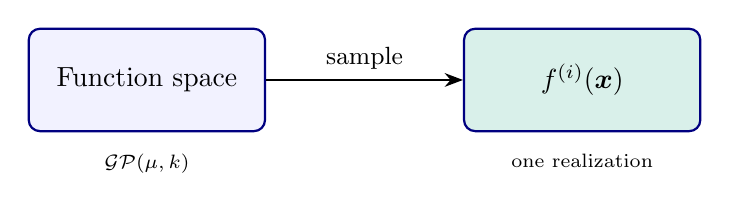
\begin{tikzpicture}[>=Stealth]
\node[draw=uzhblue, thick, rounded corners, fill=blue!5,
      minimum width=3cm, minimum height=1.3cm] (fspace) {Function space};
\node[right=2.5cm of fspace, draw=uzhblue, thick, rounded corners, fill=softgreen!15,
      minimum width=3cm, minimum height=1.3cm] (sample) {$f^{(i)}(\x)$};
\draw[->, thick] (fspace) -- node[above, font=\small] {sample} (sample);
\node[below=0.15cm of fspace, font=\scriptsize] {$\mathcal{GP}(\mu, k)$};
\node[below=0.15cm of sample, font=\scriptsize] {one realization};
\end{tikzpicture}
\end{center}
\end{frame}

% --- Kernels ---
\begin{frame}{Kernels: Where the Prior Lives}
\vspace{-0.1cm}
\begin{columns}[T]
\column{0.5\textwidth}
\begin{center}
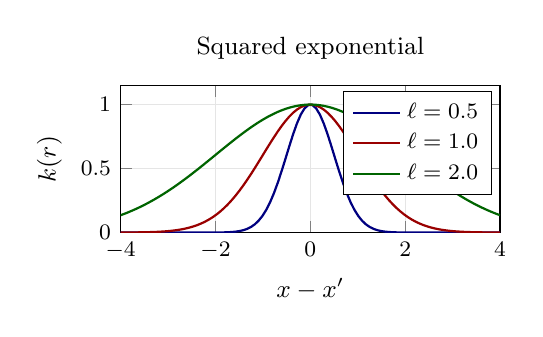
\begin{tikzpicture}
\begin{axis}[
    width=6.4cm, height=3.45cm,
    xlabel={$x - x'$}, ylabel={$k(r)$},
    xmin=-4, xmax=4, ymin=0, ymax=1.15,
    title={Squared exponential},
    legend style={at={(0.98,0.96)}, anchor=north east},
    grid=major, grid style={gray!20},
    every axis plot/.append style={thick, no markers},
]
\addplot[uzhblue, domain=-4:4, samples=100] {exp(-x^2/(2*0.5^2))};
\addlegendentry{$\ell = 0.5$}
\addplot[harvardcrimson, domain=-4:4, samples=100] {exp(-x^2/(2*1.0^2))};
\addlegendentry{$\ell = 1.0$}
\addplot[darkgreen, domain=-4:4, samples=100] {exp(-x^2/(2*2.0^2))};
\addlegendentry{$\ell = 2.0$}
\end{axis}
\end{tikzpicture}
\end{center}
{\footnotesize $k_{\mathrm{SE}}(r) = \sigma_f^2 \exp(-r^2/2\ell^2)$. Larger $\ell$ $\Rightarrow$ smoother; samples are \emphc{infinitely differentiable}, often too optimistic.}
\column{0.5\textwidth}
\begin{center}
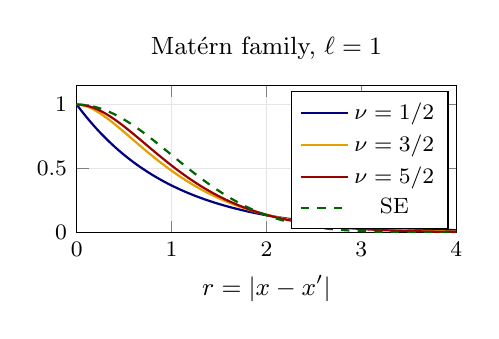
\begin{tikzpicture}
\begin{axis}[
    width=6.4cm, height=3.45cm,
    xlabel={$r = |x - x'|$},
    xmin=0, xmax=4, ymin=0, ymax=1.15,
    title={Mat\'ern family, $\ell = 1$},
    legend style={at={(0.98,0.96)}, anchor=north east},
    grid=major, grid style={gray!20},
    every axis plot/.append style={thick, no markers},
]
\addplot[uzhblue, domain=0:4, samples=200] {exp(-x)};
\addlegendentry{$\nu = 1/2$}
\addplot[softorange, domain=0:4, samples=200] {(1 + sqrt(3)*x)*exp(-sqrt(3)*x)};
\addlegendentry{$\nu = 3/2$}
\addplot[harvardcrimson, domain=0:4, samples=200] {(1 + sqrt(5)*x + 5*x^2/3)*exp(-sqrt(5)*x)};
\addlegendentry{$\nu = 5/2$}
\addplot[darkgreen, dashed, domain=0:4, samples=200] {exp(-x^2/2)};
\addlegendentry{SE}
\end{axis}
\end{tikzpicture}
\end{center}
{\footnotesize $\nu$ sets differentiability: samples are $\lceil \nu \rceil - 1$ times differentiable. \emphc{$\nu = 5/2$ is the sane default} for value and policy functions.}
\end{columns}

\vspace{0.1cm}
{\footnotesize Choosing the kernel is not a technicality: it \emph{is} the model. Assume more smoothness than the truth has, and the GP interpolates confidently straight through a kink.}
\end{frame}

% --- Posterior ---
\begin{frame}{GP Regression: The Posterior in Two Lines}
\textbf{Joint distribution of training values $\bm f$ and test values $\bm f_*$:}
\[
\begin{pmatrix} \bm f \\ \bm f_* \end{pmatrix} \sim
\mathcal{N}\!\left(\bm 0,\;
\begin{pmatrix} K & K_* \\ K_*^\top & K_{**} \end{pmatrix}\right),
\qquad K_{ij} = k(\x_i, \x_j).
\]

\textbf{Condition on what you observed}, the two lines from three slides ago:
\begin{align*}
\bm\mu_{*|\mathcal{D}} &= K_*^\top K^{-1} \bm f\\
\Sigma_{*|\mathcal{D}} &= K_{**} - K_*^\top K^{-1} K_*
\end{align*}

\vspace{0.15cm}
\begin{alertblock}{Read the variance line carefully}
\begin{itemize}\itemsep1pt
  \item Near the data: $K_*^\top K^{-1} K_* \approx K_{**}$, so the variance \emphc{collapses}.
  \item Far from the data: $K_*^\top K^{-1} K_* \approx 0$, so the variance \emphc{reverts to the prior}.
\end{itemize}
\vspace{2pt}
Note what this means: the GP \emph{knows it is extrapolating}, and says so, without ever seeing the true function out there. No trained network does this by default.
\end{alertblock}
\end{frame}

% --- Noise ---
\begin{frame}{Noise, the Nugget, and Numerical Stability}
\small
\textbf{Observation model.} If labels carry noise, $y = f(\x) + \varepsilon$ with $\varepsilon \sim \mathcal{N}(0,\sigma_y^2)$, then $\mathrm{cov}[y_p, y_q] = k(\x_p,\x_q) + \sigma_y^2 \delta_{pq}$, so everywhere replace $K$ by $K_y = K + \sigma_y^2 I$:
\[
\bar f_* = \bm k_*^\top (K + \sigma_y^2 I)^{-1} \bm y,
\qquad
\sigma_*^2 = k(\x_*,\x_*) - \bm k_*^\top (K + \sigma_y^2 I)^{-1} \bm k_* .
\]

\vspace{0.2cm}
\begin{columns}[T]
\column{0.47\textwidth}
\textbf{Noiseless} ($\sigma_y^2 = 0$)
\begin{itemize}\itemsep1pt
  \item Interpolates the training points exactly
  \item Variance is zero at training inputs
  \item Needs $K$ strictly positive definite
\end{itemize}
\column{0.5\textwidth}
\textbf{Noisy} ($\sigma_y^2 > 0$)
\begin{itemize}\itemsep1pt
  \item Smooths through the training points
  \item Variance positive everywhere
  \item Much better conditioned
\end{itemize}
\end{columns}

\vspace{0.25cm}
\begin{block}{In practice}
Even for a ``noiseless'' surrogate, add a jitter of $\sigma_y^2 \sim 10^{-6}$. \emphc{And be honest about whether it really is noiseless}: if the labels came from a Monte Carlo simulation or an iterative solver stopped at a tolerance, they carry noise, and pretending otherwise makes the Cholesky factorization fail before it makes the statistics wrong.
\end{block}
\end{frame}

% --- Prediction and credible bands ---
\begin{frame}{Prediction and Credible Bands}
\begin{center}
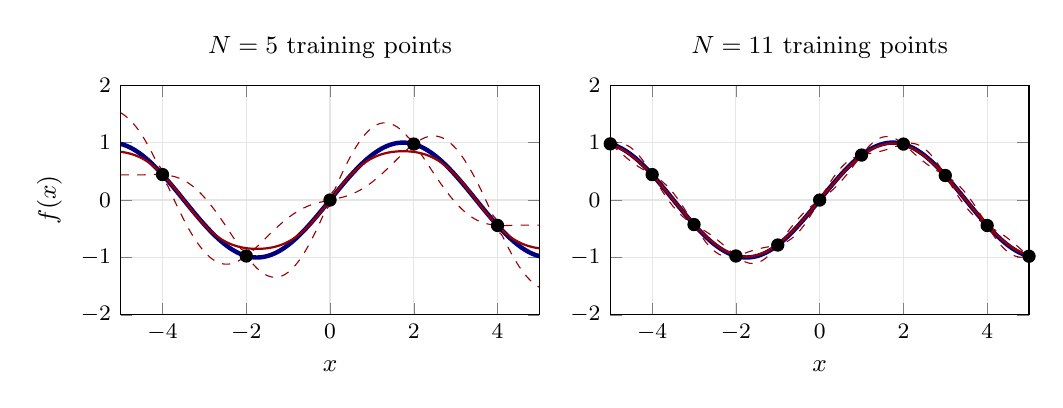
\begin{tikzpicture}
\begin{axis}[
    name=left,
    width=6.9cm, height=4.5cm,
    title={$N = 5$ training points},
    xlabel={$x$}, ylabel={$f(x)$},
    xmin=-5, xmax=5, ymin=-2, ymax=2,
    grid=major, grid style={gray!20},
    every axis plot/.append style={no markers},
]
\addplot[uzhblue, ultra thick, domain=-5:5, samples=200] {sin(deg(0.9*x))};
\addplot[harvardcrimson, thick, domain=-5:5, samples=200] {0.90*sin(deg(0.9*x)) + 0.05*sin(deg(2.7*x))};
\addplot[harvardcrimson, thin, dashed, domain=-5:5, samples=400]
    {sin(deg(0.9*x)) + 0.6*sqrt( max(1 - exp(-(x+4)^2/0.6) - exp(-(x+2)^2/0.6) - exp(-(x-0)^2/0.6) - exp(-(x-2)^2/0.6) - exp(-(x-4)^2/0.6), 0.02) )};
\addplot[harvardcrimson, thin, dashed, domain=-5:5, samples=400]
    {sin(deg(0.9*x)) - 0.6*sqrt( max(1 - exp(-(x+4)^2/0.6) - exp(-(x+2)^2/0.6) - exp(-(x-0)^2/0.6) - exp(-(x-2)^2/0.6) - exp(-(x-4)^2/0.6), 0.02) )};
\addplot[only marks, mark=*, mark size=2.2pt, black] coordinates {(-4,0.443) (-2,-0.974) (0,0) (2,0.974) (4,-0.443)};
\end{axis}

\begin{axis}[
    at={(left.east)}, anchor=west, xshift=0.9cm,
    width=6.9cm, height=4.5cm,
    title={$N = 11$ training points},
    xlabel={$x$},
    xmin=-5, xmax=5, ymin=-2, ymax=2,
    grid=major, grid style={gray!20},
    every axis plot/.append style={no markers},
]
\addplot[uzhblue, ultra thick, domain=-5:5, samples=200] {sin(deg(0.9*x))};
\addplot[harvardcrimson, thick, domain=-5:5, samples=200] {0.985*sin(deg(0.9*x))};
\addplot[harvardcrimson, thin, dashed, domain=-5:5, samples=400]
    {sin(deg(0.9*x)) + 0.15*sqrt( max(1 - exp(-(x+5)^2/0.15) - exp(-(x+4)^2/0.15) - exp(-(x+3)^2/0.15) - exp(-(x+2)^2/0.15) - exp(-(x+1)^2/0.15) - exp(-x^2/0.15) - exp(-(x-1)^2/0.15) - exp(-(x-2)^2/0.15) - exp(-(x-3)^2/0.15) - exp(-(x-4)^2/0.15) - exp(-(x-5)^2/0.15), 0.05) )};
\addplot[harvardcrimson, thin, dashed, domain=-5:5, samples=400]
    {sin(deg(0.9*x)) - 0.15*sqrt( max(1 - exp(-(x+5)^2/0.15) - exp(-(x+4)^2/0.15) - exp(-(x+3)^2/0.15) - exp(-(x+2)^2/0.15) - exp(-(x+1)^2/0.15) - exp(-x^2/0.15) - exp(-(x-1)^2/0.15) - exp(-(x-2)^2/0.15) - exp(-(x-3)^2/0.15) - exp(-(x-4)^2/0.15) - exp(-(x-5)^2/0.15), 0.05) )};
\addplot[only marks, mark=*, mark size=2.2pt, black] coordinates
    {(-5,0.978) (-4,0.443) (-3,-0.427) (-2,-0.974) (-1,-0.783) (0,0)
     (1,0.783) (2,0.974) (3,0.427) (4,-0.443) (5,-0.978)};
\end{axis}
\end{tikzpicture}
\end{center}

\vspace{0.05cm}
{\footnotesize \textcolor{uzhblue}{\textbf{Blue:}} true function. \textcolor{harvardcrimson}{\textbf{Red:}} posterior mean. \textcolor{harvardcrimson}{\textbf{Dashed:}} approximate 95\% credible band. The band pinches shut at each training input and balloons between them, and \emphc{that shape is the map of where to sample next}, and we use it at the end of this part.}
\end{frame}

% --- Length scale ---
\begin{frame}{Getting the Length Scale Wrong}
\begin{center}
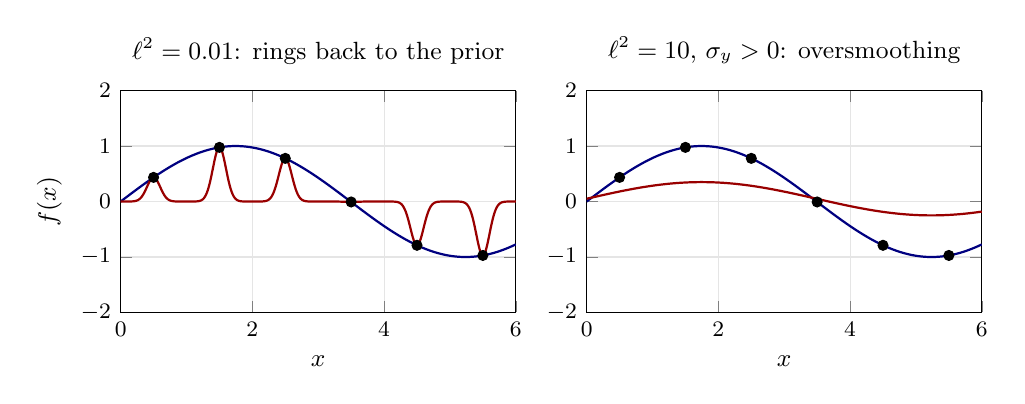
\begin{tikzpicture}
\begin{axis}[
    name=p1,
    width=6.6cm, height=4.4cm,
    title={$\ell^2 = 0.01$: rings back to the prior},
    xlabel={$x$}, ylabel={$f(x)$},
    xmin=0, xmax=6, ymin=-2, ymax=2,
    grid=major, grid style={gray!20},
    every axis plot/.append style={no markers},
]
\addplot[uzhblue, thick, domain=0:6, samples=200] {sin(deg(0.9*x))};
\addplot[harvardcrimson, thick, domain=0:6, samples=400]
    {0.435*exp(-(x-0.5)^2/0.02) + 0.976*exp(-(x-1.5)^2/0.02)
   + 0.778*exp(-(x-2.5)^2/0.02) - 0.008*exp(-(x-3.5)^2/0.02)
   - 0.789*exp(-(x-4.5)^2/0.02) - 0.972*exp(-(x-5.5)^2/0.02)};
\addplot[only marks, mark=*, mark size=1.8pt, black] coordinates
    {(0.5,0.435) (1.5,0.976) (2.5,0.778) (3.5,-0.008) (4.5,-0.789) (5.5,-0.972)};
\end{axis}

\begin{axis}[
    at={(p1.east)}, anchor=west, xshift=0.9cm,
    width=6.6cm, height=4.4cm,
    title={$\ell^2 = 10$, $\sigma_y > 0$: oversmoothing},
    xlabel={$x$},
    xmin=0, xmax=6, ymin=-2, ymax=2,
    grid=major, grid style={gray!20},
    every axis plot/.append style={no markers},
]
\addplot[uzhblue, thick, domain=0:6, samples=200] {sin(deg(0.9*x))};
\addplot[harvardcrimson, thick, domain=0:6, samples=200] {0.30*sin(deg(0.9*x)) + 0.05};
\addplot[only marks, mark=*, mark size=1.8pt, black] coordinates
    {(0.5,0.435) (1.5,0.976) (2.5,0.778) (3.5,-0.008) (4.5,-0.789) (5.5,-0.972)};
\end{axis}
\end{tikzpicture}
\end{center}

\vspace{0.1cm}
\small
\begin{columns}[T]
\column{0.48\textwidth}
\textbf{Too short.} The GP interpolates every point exactly and then \emphc{falls back to the prior mean in between}. Perfect training fit, useless predictions, and the credible band (previous slide) balloons in exactly those gaps.
\column{0.48\textwidth}
\textbf{Too long.} The posterior mean flattens and no longer passes through the data. The band is narrow and \emphc{confidently wrong}, which is the more dangerous failure of the two.
\end{columns}
\end{frame}

% --- Hyperparameters ---
\begin{frame}{Learning the Hyperparameters, and a Free Diagnostic}
\small
\begin{block}{Marginal likelihood: how $\ell$, $\sigma_f$, $\sigma_y$ get chosen}
\vspace{-6pt}
\[
\log p(\bm y \mid X) =
\underbrace{-\tfrac{1}{2}\bm y^\top K_y^{-1} \bm y}_{\text{data fit}}
\underbrace{-\tfrac{1}{2}\log|K_y|}_{\text{complexity penalty}}
\underbrace{-\tfrac{N}{2}\log(2\pi)}_{\text{constant}}
\]
\vspace{-8pt}

The two terms pull against each other: \emphc{an automatic Occam's razor}, with closed-form gradients and no validation split spent. Optimize with restarts; it is multimodal.
\end{block}

\vspace{0.08cm}
\begin{block}{Leave-one-out, for free}
\vspace{-6pt}
\[
\mu_{-i}(\x_i) - y_i = -\frac{[K_y^{-1}\bm y]_i}{[K_y^{-1}]_{ii}},
\qquad
\sigma^2_{-i}(\x_i) = \frac{1}{[K_y^{-1}]_{ii}} .
\]
\vspace{-8pt}

These need $\mathrm{diag}(K_y^{-1})$, so \emph{all $N$} leave-one-out residuals cost one further $\mathcal{O}(N^3)$ solve, the same order you already paid, and \emphc{no refitting and no held-out data}. Doing $N$ honest refits would be $\mathcal{O}(N^4)$. \emphc{This is the number to report for a surrogate}; Part V quotes it.
\end{block}

\vspace{0.1cm}
{\footnotesize Closed form: Rasmussen \& Williams (2006), \S\,5.4.2, in \texttt{../readings}.}
\end{frame}

% --- Code ---
\begin{frame}[fragile]{GP Regression in Fifteen Lines}
\begin{lstlisting}[basicstyle=\scriptsize\ttfamily]
import numpy as np
from scipy.linalg import cho_factor, cho_solve

def kernel(X1, X2, l=1.0, sf=1.0):
    sq = np.sum(X1**2, 1).reshape(-1, 1) \
         + np.sum(X2**2, 1) - 2 * X1 @ X2.T
    return sf**2 * np.exp(-0.5 * sq / l**2)

K = kernel(X_tr, X_tr) + 1e-8 * np.eye(N)   # jitter
L, low = cho_factor(K, lower=True)          # O(N^3), once
alpha  = cho_solve((L, low), y_tr)          # the weights

Ks  = kernel(X_tr, X_te)
mu  = Ks.T @ alpha                          # posterior mean
v   = cho_solve((L, low), Ks)
var = kernel(X_te, X_te) - Ks.T @ v         # posterior variance
\end{lstlisting}

\vspace{0.1cm}
{\footnotesize No training loop, no learning rate, no architecture: the whole model is the kernel and one Cholesky factorization. Compare Algorithm 2.1 in Rasmussen \& Williams (2006); notebook \texttt{03\_02} builds this and checks it against \texttt{sklearn}.}
\end{frame}

% --- Complexity ---
\begin{frame}{What It Costs: $\mathcal{O}(N^3)$}
\small
\begin{block}{Cost of exact GP inference}
\begin{itemize}\itemsep1pt
  \item \textbf{Fitting:} Cholesky of $K_y \in \R^{N\times N}$: \emphc{$\mathcal{O}(N^3)$} time, $\mathcal{O}(N^2)$ memory.
  \item \textbf{Prediction:} $\mathcal{O}(N)$ per test point (mean), $\mathcal{O}(N^2)$ (variance).
  \item \textbf{Hyperparameters:} $\mathcal{O}(N^3)$ per step.
\end{itemize}
\end{block}

\vspace{0.05cm}
\begin{block}{If you really need large $N$}
Sparse GPs (inducing points, rank $M \ll N$, cost $\mathcal{O}(NM^2)$), random Fourier features, GPyTorch.
\end{block}

\vspace{0.05cm}
\begin{alertblock}{But notice where this bites}
The cubic cost sounds fatal until you ask \emph{why} $N$ is small. \emphc{If a label costs a four-hour solve, you were never reaching $N = 10^4$ anyway.} The regime where GPs are cheap to fit is the regime where data is expensive to get.
\end{alertblock}
\end{frame}

% --- GP vs DNN ---
\begin{frame}{Gaussian Processes versus Deep Networks}
\begin{center}
\scriptsize
\setlength{\tabcolsep}{4pt}
\begin{tabular}{l l l}
\toprule
\textbf{Criterion} & \textbf{Gaussian process} & \textbf{Deep neural network} \\
\midrule
Uncertainty & \yes built in (posterior variance) & \no needs ensembles or MC dropout \\
Hyperparameters & \yes marginal likelihood & \mixed search: random, Hyperband \\
Scaling in $N$ & \no $\mathcal{O}(N^3)$, practical limit ${\sim}10^4$ & \yes $\mathcal{O}(N)$ per epoch \\
Scaling in $d$ & \no degrades past $d \approx 10$ & \yes handles $d \gg 100$ \\
Small data ($N < 100$) & \yes excellent & \no underfits, or memorizes \\
Fitting & \yes closed form & \mixed SGD, many epochs, seed-dependent \\
Interpretability & \yes the kernel \emph{is} the assumption & \no black box \\
\bottomrule
\end{tabular}
\end{center}

\vspace{0.15cm}
\begin{alertblock}{The decision rule is the \emph{cost of a label}, not taste}
\small
\begin{itemize}\itemsep1pt
  \item \textbf{Labels cheap, $d$ large:} \emphc{deep network}, as in Part II's option-pricing surrogate.
  \item \textbf{Labels expensive, $d \lesssim 10$:} \emphc{GP plus active learning}, as in Parts IV and V. (The table's ``degrades past $d \approx 10$'' is the same boundary.)
  \item \textbf{Both, layered:} a DEQN solves the equilibrium, a GP maps its output to the QoI.
\end{itemize}
\end{alertblock}
\end{frame}

% --- Finger exercise ---
\begin{frame}{Finger Exercise: How Many Points?}
\begin{flushright}\exercisepause{}\end{flushright}
\vspace{-0.35cm}
\begin{exampleblock}{The setting}
You must map a welfare objective over a \emphc{6-dimensional} policy box. One evaluation means simulating a stochastic OLG model, $\approx 4$ hours of wall-clock time. You have a 64-core machine and \emphc{two weeks}.
\end{exampleblock}

\vspace{0.4cm}
\begin{enumerate}\itemsep6pt
  \item Roughly how many evaluations can you afford?
  \item How many points per dimension would a tensor grid give you at that budget?
  \item Which approximator does that budget select, and why?
\end{enumerate}
\end{frame}

\begin{frame}{Solution: How Many Points?}
\small
\begin{block}{1. The budget}
$14 \text{ days} \times 24 \text{ h} = 336$ h of wall-clock time; at 64 cores that is ${\sim}21{,}500$ core-hours, so about \emphc{5{,}000 evaluations} at 4 h each. Call it a few thousand, allowing for failures and re-runs.
\end{block}

\begin{block}{2. What a grid does with them}
$5{,}376^{1/6} \approx 4.2$ points per dimension. Four per axis will not resolve a curved welfare surface, and refining to a still-inadequate six costs $6^6 = 46{,}656$ evaluations $= 187{,}000$ core-hours, or \emphc{four months} on the same 64 cores (21 years on one).
\end{block}

\begin{block}{3. Which approximator}
A few thousand points is far too few to train a deep network, and comfortably inside the $\mathcal{O}(N^3)$ range of an exact GP. \emphc{Choose the GP}, and since every point is precious, do not place them on a grid at all. Let the posterior variance choose them.
\end{block}

\vspace{0.1cm}
{\footnotesize The real study in Part V spent \emphc{500}, not 5{,}000. The next three slides are how.}
\end{frame}

% --- BAL idea ---
\begin{frame}{Where to Sample Next}
\small
\begin{columns}[T]
\column{0.48\textwidth}
\textbf{Fixed design}
\begin{itemize}\itemsep1pt
  \item Spread evenly, fixed before you know anything
  \item Wasted where the function is flat
\end{itemize}
\column{0.48\textwidth}
\textbf{Active design}
\begin{itemize}\itemsep1pt
  \item Goes where the surrogate is \emphc{uncertain}
  \item Reuses the posterior variance you already have
\end{itemize}
\end{columns}

\vspace{-0.02cm}
\begin{block}{The score function}
\vspace{-6pt}
\[
U(\x) = w_{\mathrm{obj}}\, \mu(\x) + \frac{w_{\mathrm{var}}}{2}\,\log \sigma^2(\x)
\]
\vspace{-8pt}
\begin{itemize}\itemsep1pt
  \item $\sigma^2(\x)$, \emphc{exploration}: sample where the variance is large.
  \item $\mu(\x)$, \emphc{objective-following}: for Bayesian \emph{optimization}.
\end{itemize}
\end{block}

\vspace{0.02cm}
{\footnotesize \textbf{In practice} Part V uses the upper-confidence-bound form $\alpha = \lambda\mu + \kappa\sigma$, $\lambda = 1$, $\kappa = 100$: exploration-weighted, but not pure, because there the optimum \emph{is} the target. \emphc{And note what $\sigma^2$ does not depend on:} with hyperparameters fixed it is a function of the \emph{design} alone, for any kernel. Refit $\ell$ each step and the data creep back in; two slides on, that matters.}
\end{frame}

% --- BAL algorithm ---
\begin{frame}{The BAL Algorithm}
\begin{block}{Bayesian active learning for surrogates}
\begin{algorithmic}[1]
\REQUIRE initial design $\mathcal{D}_0 = \{(\x_i, y_i)\}_{i=1}^{n_0}$, budget $N$, candidate set $\mathcal{C}$
\STATE fit a GP on $\mathcal{D}_0$, giving $\mu(\cdot)$ and $\sigma^2(\cdot)$
\FOR{$t = 1, \dots, N - n_0$}
  \STATE evaluate $U(\x) = w_{\mathrm{obj}}\,\mu(\x) + \tfrac{w_{\mathrm{var}}}{2}\log\sigma^2(\x)$ for all $\x \in \mathcal{C}$
  \STATE select $\x_{\mathrm{new}} = \argmax_{\x \in \mathcal{C}} U(\x)$
  \STATE \emphc{query the expensive model:} $y_{\mathrm{new}} = f(\x_{\mathrm{new}})$
  \STATE update $\mathcal{D}_t \leftarrow \mathcal{D}_{t-1} \cup \{(\x_{\mathrm{new}}, y_{\mathrm{new}})\}$ and refit the GP
\ENDFOR
\RETURN the trained GP surrogate
\end{algorithmic}
\end{block}

\vspace{0.05cm}
{\footnotesize Scheidegger \& Bilionis (2019), in \texttt{../readings}, puts this loop to work on economic models.}

\vspace{0.15cm}
{\footnotesize Every step except line 5 is cheap; the loop exists to make line 5 happen as rarely as possible, and in a real study to tolerate its failure.}
\end{frame}

% --- BAL in action ---
\begin{frame}{BAL in Action}
\small Each new point goes where the posterior variance is largest (the marked point).\par\normalsize

\vspace{-0.05cm}
\begin{center}
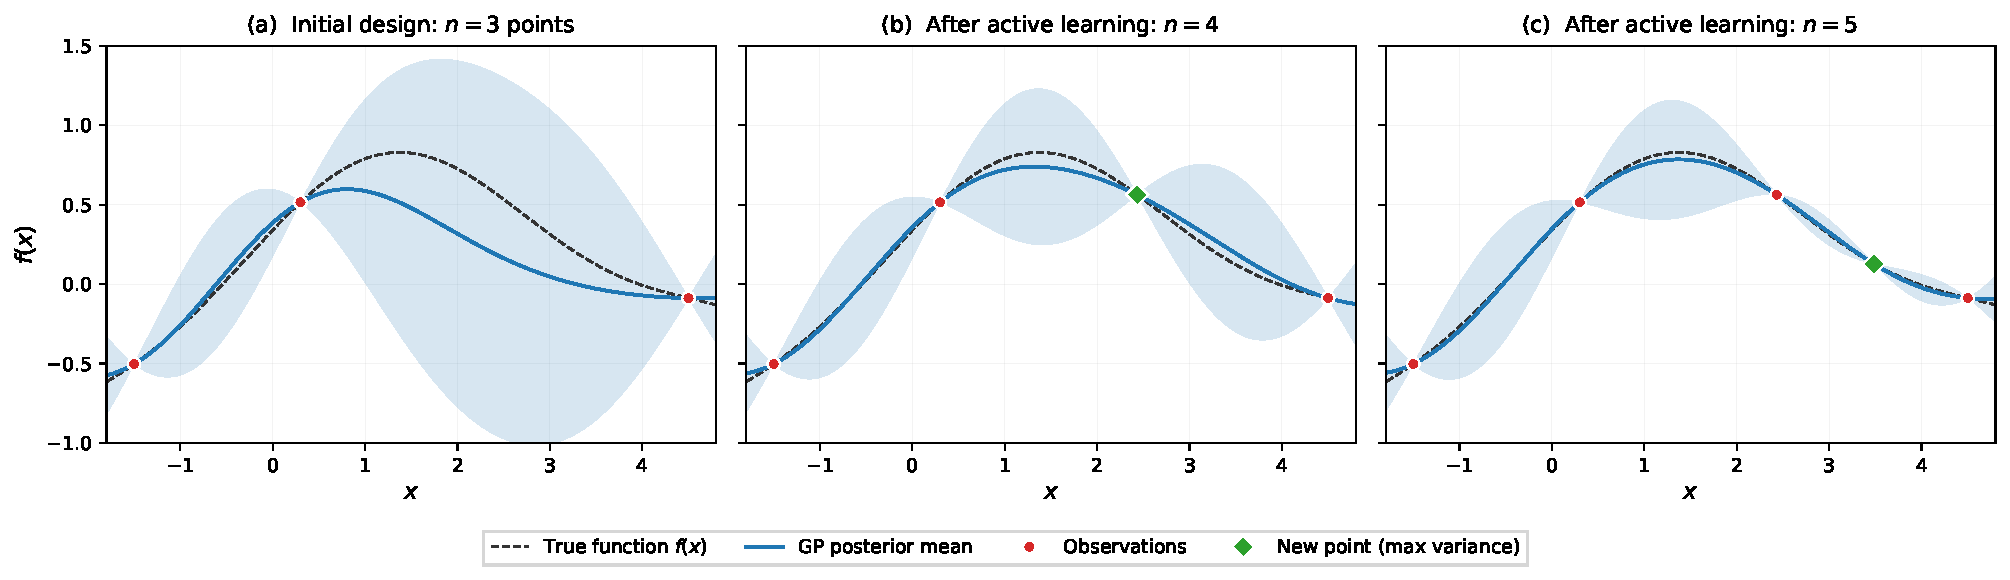
\includegraphics[width=0.89\textwidth]{figures/gp_active_learning.pdf}
\end{center}

\vspace{-0.35cm}
{\footnotesize
\textbf{(a)} three observations, the posterior drifting where there is no data. \textbf{(b)} the acquisition takes the max-variance point. \textbf{(c)} one more fills the gap: \emphc{five points suffice}.

\vspace{2pt}
\emphc{But do not oversell it.} Notebook \texttt{03\_02} runs this against a uniform design and they finish \emph{level} (MAE $0.0234$ vs $0.0237$ at $N=25$). For a \emph{stationary} kernel the posterior variance depends on the design alone, so on an interval uncertainty sampling essentially \emph{is} a space-filling design. It earns its keep where no such design exists: \emphc{irregular domains, ARD kernels, and dimensions where a grid is impossible}.}
\end{frame}

% ============================================================================
% PART IV: UNCERTAINTY QUANTIFICATION
% ============================================================================

\section{Quantify: Uncertainty}

\begin{frame}{}
\begin{center}
{\Huge \textcolor{uzhblue}{Part IV}}\\[0.8em]
{\LARGE Quantify: Uncertainty}
\end{center}
\end{frame}

% --- Motivation ---
\begin{frame}{How Uncertain Is the Social Cost of Carbon?}
\small
\begin{itemize}\itemsep3pt
  \item Carbon taxation is the consensus policy response, and the level of the tax is anchored on the \textbf{social cost of carbon} (SCC): the marginal welfare loss from one extra tonne of CO$_2$.
  \item The SCC is computed inside \textbf{integrated assessment models} (IAMs), coupling an economy to a climate system.
  \item Those models carry serious \emphc{parametric} uncertainty: the equilibrium climate sensitivity, the damage function, risk aversion, the discount rate, on top of stochastic tipping risk.
\end{itemize}

\vspace{0.15cm}
\begin{alertblock}{The question, and the wall}
Not ``what is the SCC?'' but \emphc{``which uncertainties actually drive it?''}, because that tells a modeler where to spend the next year of work and a policymaker which number to scrutinize.

\vspace{2pt}
Answering it globally means propagating a distribution over parameters through the model. One-at-a-time perturbations are \emph{local} and depend entirely on where you happened to start.
\end{alertblock}

\vspace{0.1cm}
{\footnotesize Friedl, K\"ubler, Scheidegger \& Usui (2023), \emph{Deep Uncertainty Quantification}, in \texttt{../readings}.}
\end{frame}

% --- Parameters as pseudo-states ---
\begin{frame}{Uncertain Parameters as Pseudo-States}
\small
\begin{columns}[T]
\column{0.44\textwidth}
\begin{center}
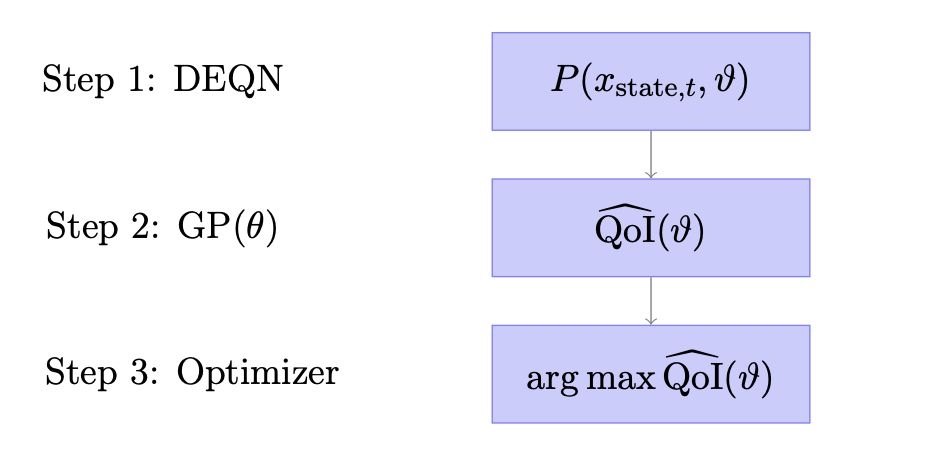
\includegraphics[width=\linewidth]{figures/flow_chart_2.png}
\end{center}
\column{0.54\textwidth}
\begin{enumerate}\itemsep2pt
  \item \textbf{Surrogate 1.} A DEQN solves the IAM globally, with the uncertain $\str$ carried as pseudo-states, the move Part II made with $\varrho$. \emphc{One model solve, not one per draw.}
  \item \textbf{Simulate.} Draw $N$ parameter vectors, simulate under the learned policies, record the quantity of interest, $\mathrm{SCC}(\str)$.
  \item \textbf{Surrogate 2.} Fit a cheap approximation to $\str \mapsto \mathrm{SCC}(\str)$ from those $N$ points.
  \item \textbf{Post-process.} Univariate effects, Sobol' indices, Shapley values, millions of queries of surrogate~2, at zero cost.
\end{enumerate}
\end{columns}

\vspace{0.1cm}
\emphc{Step 3 is where Part III pays off.} $N$ is a few hundred: each point is a full model simulation. Far too few for a deep network, comfortably inside the range of an exact GP. \emphc{Surrogate~2 here is a Gaussian process.}
\end{frame}

% --- Three quantities ---
\begin{frame}{Global Sensitivity Analysis: Three Quantities}
\small
Let the quantity of interest be $y = Q(\theta_1,\dots,\theta_p)$, with $\str$ distributed over its uncertainty range.

\vspace{0.15em}
\begin{block}{Univariate effect: \emph{direction}}
\vspace{-6pt}
\[
\mathcal{M}^{1}_{i}(t) = \mathbb{E}_{\str_{-i}}\bigl[\, y \mid \theta_i = t \,\bigr]
\]
\vspace{-8pt}

How $y$ moves as $\theta_i$ sweeps its range, averaging over the rest. Answers ``\emph{which way}?''
\end{block}

\begin{block}{Sobol' index: \emph{prioritization}}
\vspace{-6pt}
\[
S_i = \frac{\mathrm{Var}_{\theta_i}\bigl[\, \mathbb{E}_{\str \setminus \theta_i}[\, y \mid \theta_i \,] \,\bigr]}{\mathrm{Var}_{\str}[\,y\,]} \in [0,1]
\]
\vspace{-8pt}

The variance share removed if $\theta_i$ were known. The \emph{total} index $S_i^{T}$ adds every interaction it takes part in. \emphc{Screening rule: fix $\theta_i$ only if $S_i^{T} < 1\%$}: a small first-order $S_i$ is not enough, since a parameter can matter entirely through interactions.
\end{block}

\vspace{0.1em}
{\footnotesize \textbf{Shapley value} (\emph{attribution}): splits the variance fairly under interactions, so shares sum to one; first-order Sobol' need not. \emphc{The results two slides on are Shapley values.}}
\end{frame}

% --- SCC distribution ---
\begin{frame}{The Quantity of Interest: SCC in \$/tonC}
\begin{columns}[c]
\column{0.49\textwidth}
\begin{center}
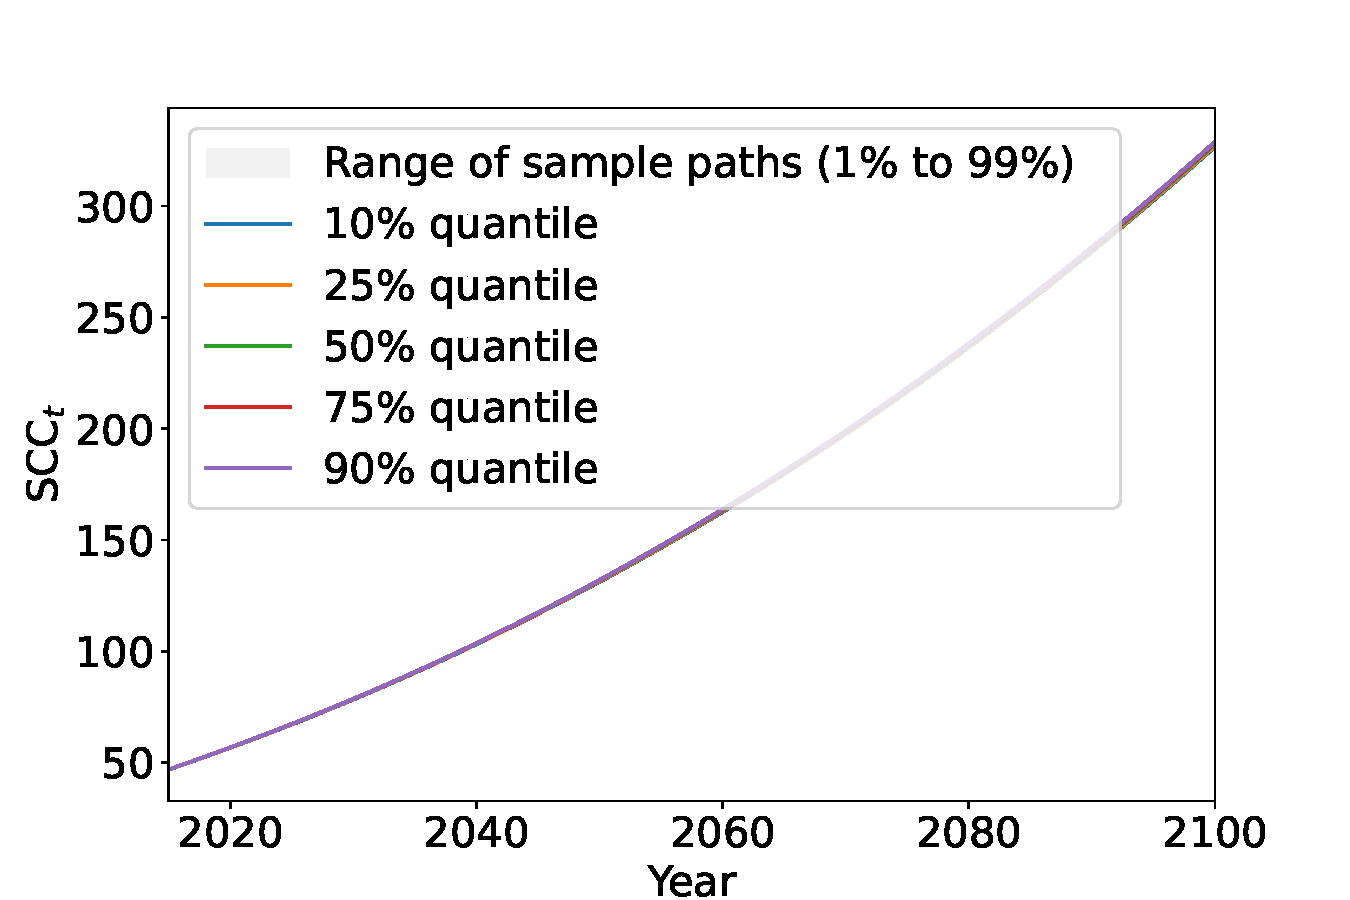
\includegraphics[width=0.94\linewidth]{figures/scc_distribution_nolearn.pdf}\\[2pt]
{\footnotesize without Bayesian learning}
\end{center}
\column{0.49\textwidth}
\begin{center}
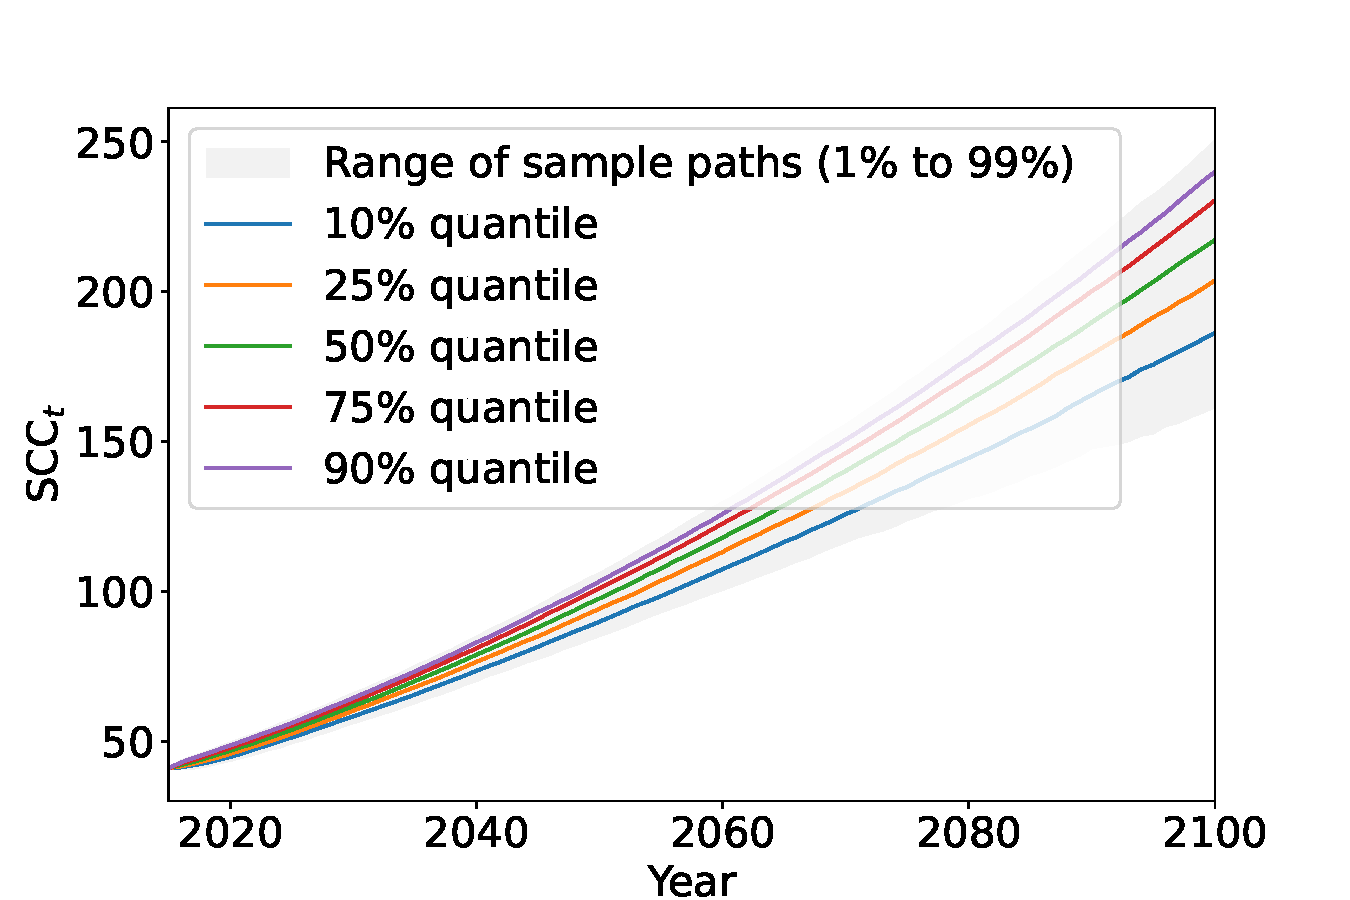
\includegraphics[width=0.94\linewidth]{figures/scc_distribution_learning.pdf}\\[2pt]
{\footnotesize with Bayesian learning}
\end{center}
\end{columns}

\vspace{0.2cm}
{\footnotesize The SCC is not a number, it is a \emphc{random variable}. Without learning the quantiles nearly coincide: beliefs are fixed, so the path is near-deterministic. With Bayesian updating they \emphc{fan out}: beliefs become a stochastic state and the SCC inherits it. \emphc{Learning adds dispersion rather than removing it.}}
\end{frame}

% --- Univariate effects ---
\begin{frame}{Univariate Effects on the SCC in 2020}
\begin{center}
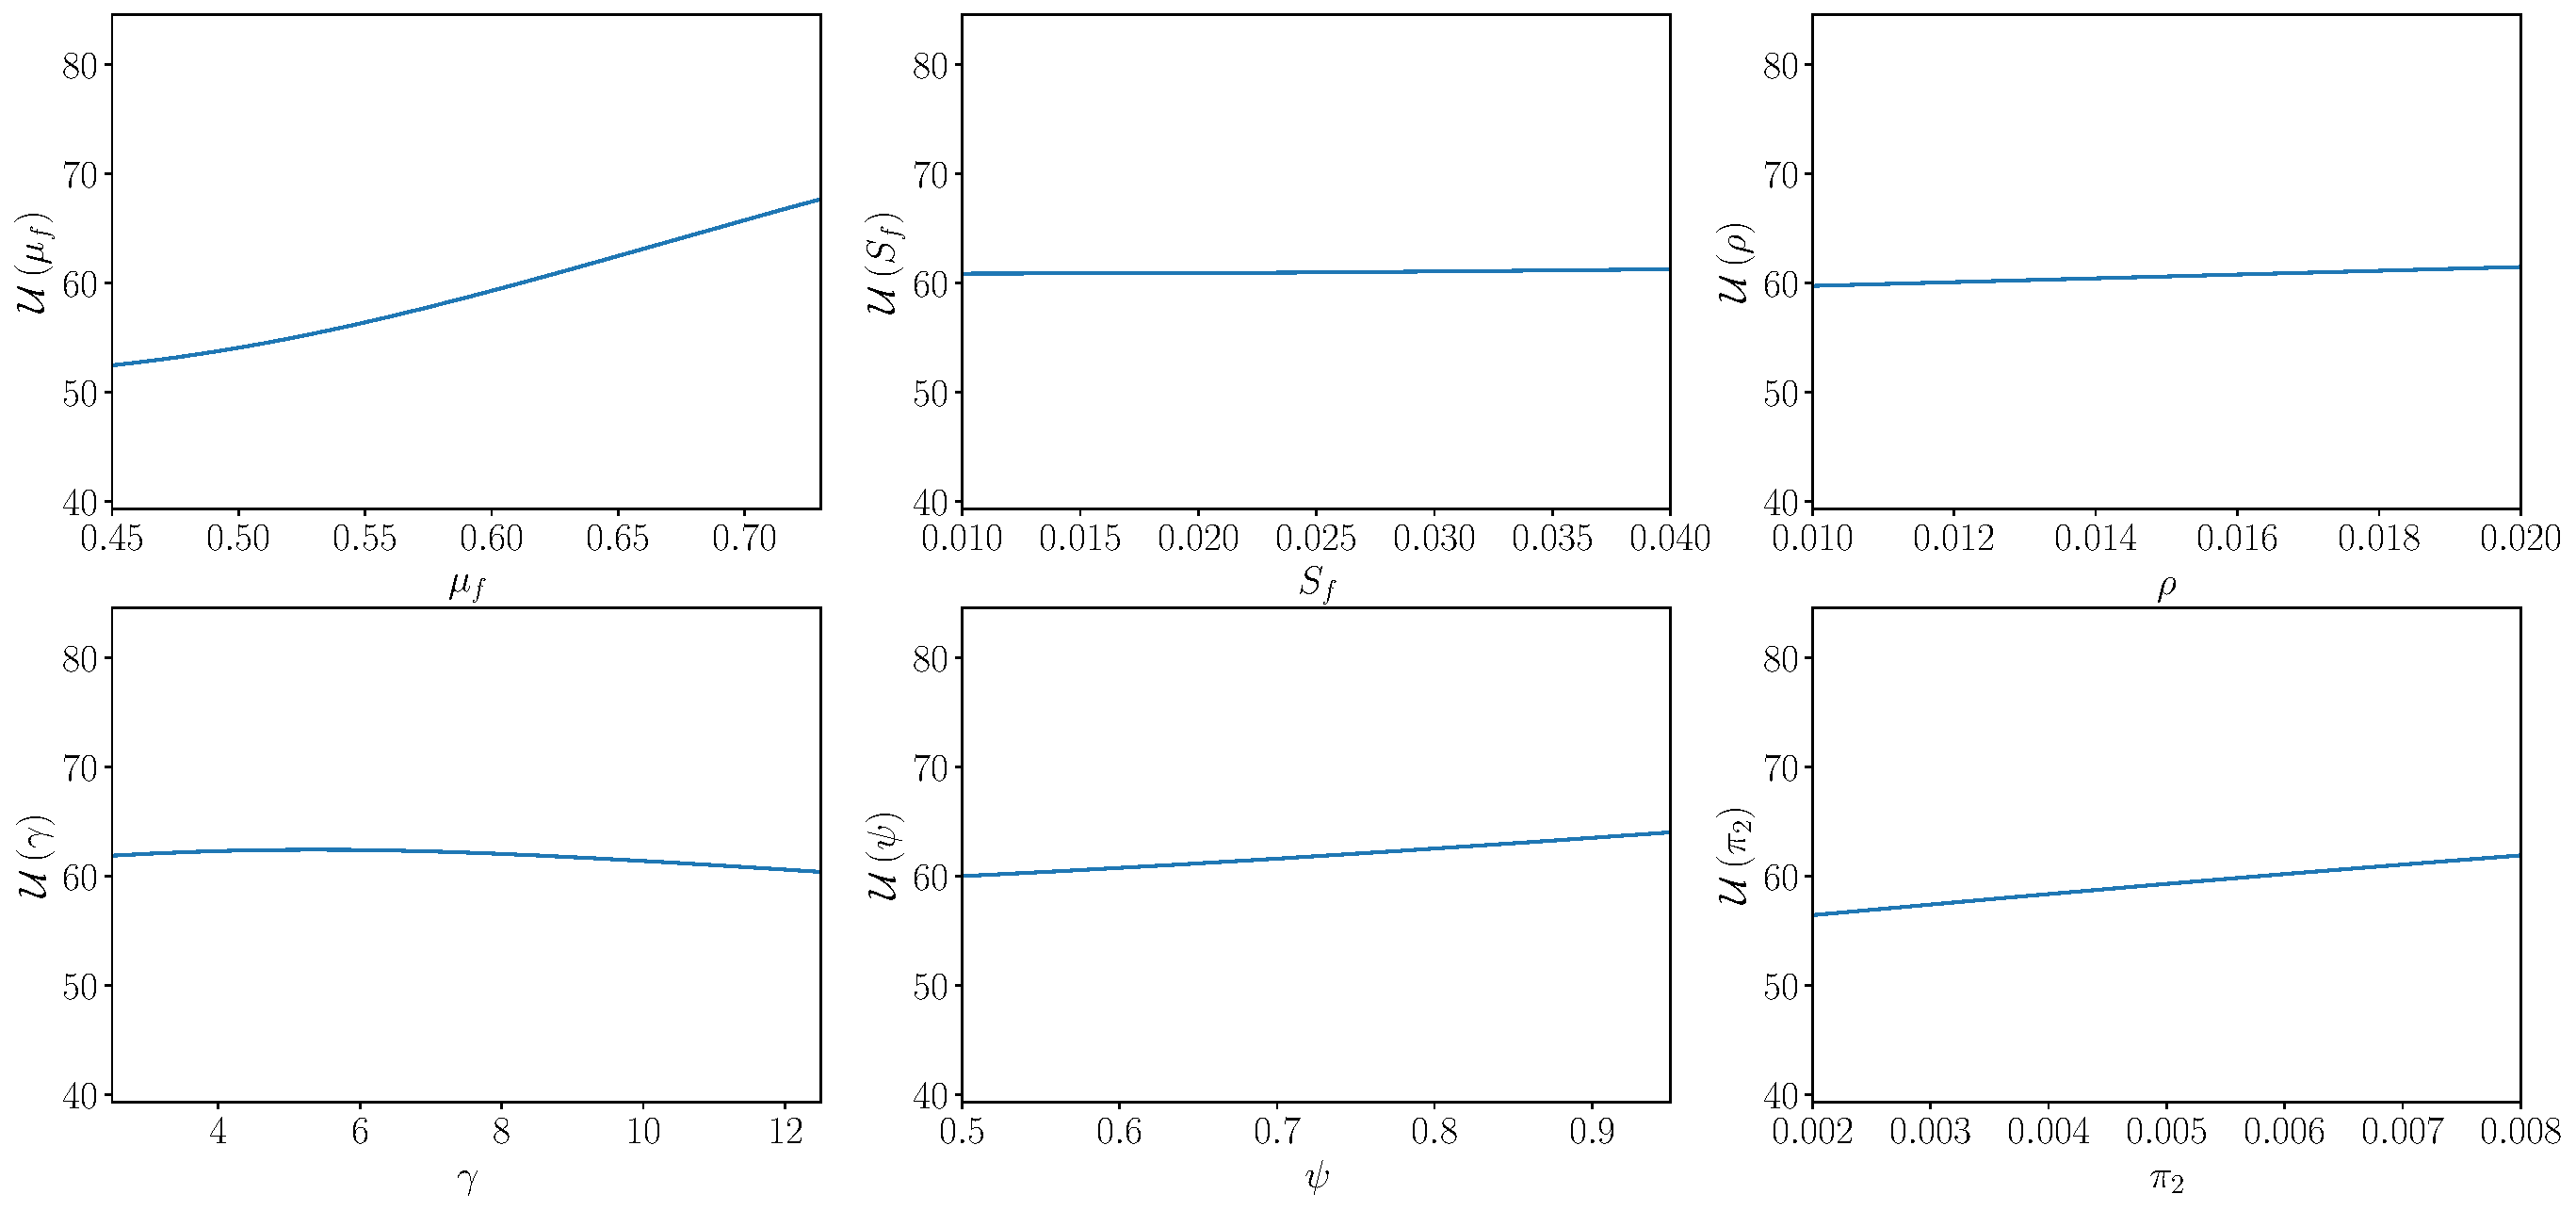
\includegraphics[width=0.84\textwidth]{figures/uni_pred_E_scc2020_panel.pdf}
\end{center}
\vspace{-0.15cm}
{\footnotesize Each panel sweeps one uncertain parameter across its range, integrating out the rest. \emphc{Flat panels are parameters you may as well calibrate}; steep and \emph{curved} panels are where the answer depends on a value nobody has pinned down, and where the next modeling effort should go.}
\end{frame}

% --- Shapley ---
\begin{frame}{What Drives the Variance: Shapley and Sobol'}
\begin{columns}[c]
\column{0.49\textwidth}
\begin{center}
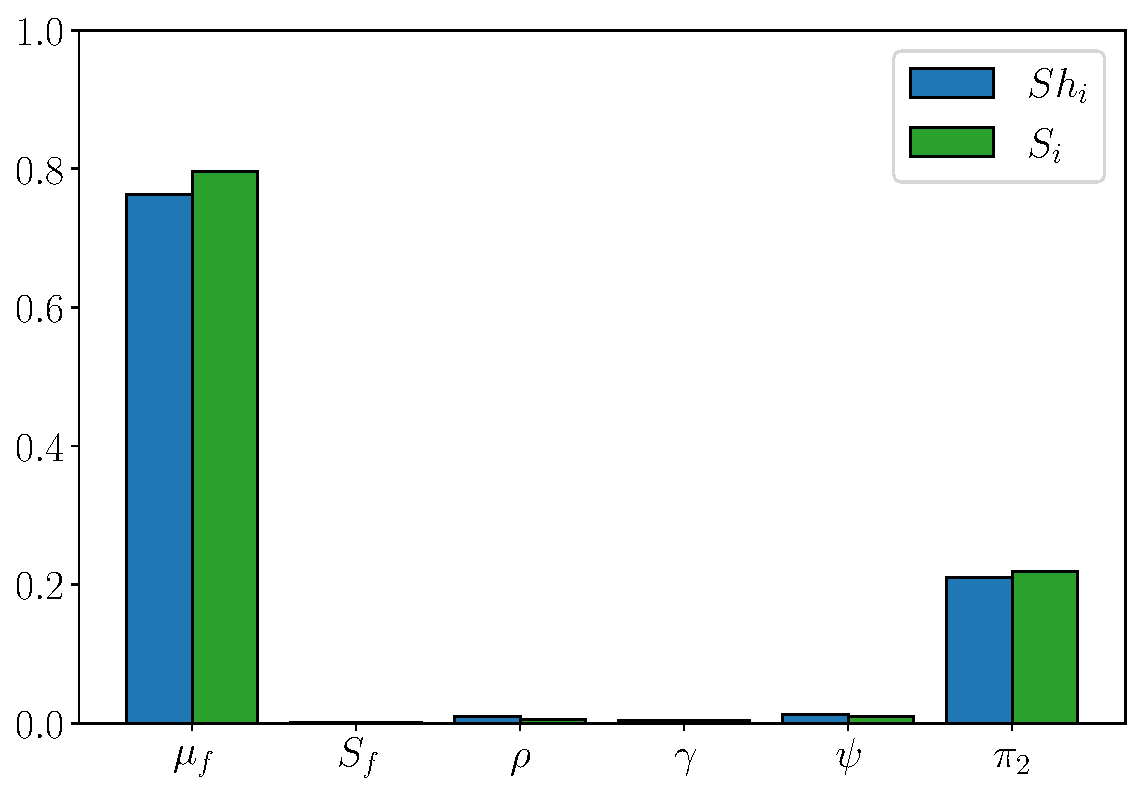
\includegraphics[width=\linewidth]{figures/scc_shapley_nolearn.pdf}\\[2pt]
{\scriptsize no learning}
\end{center}
\column{0.49\textwidth}
\begin{center}
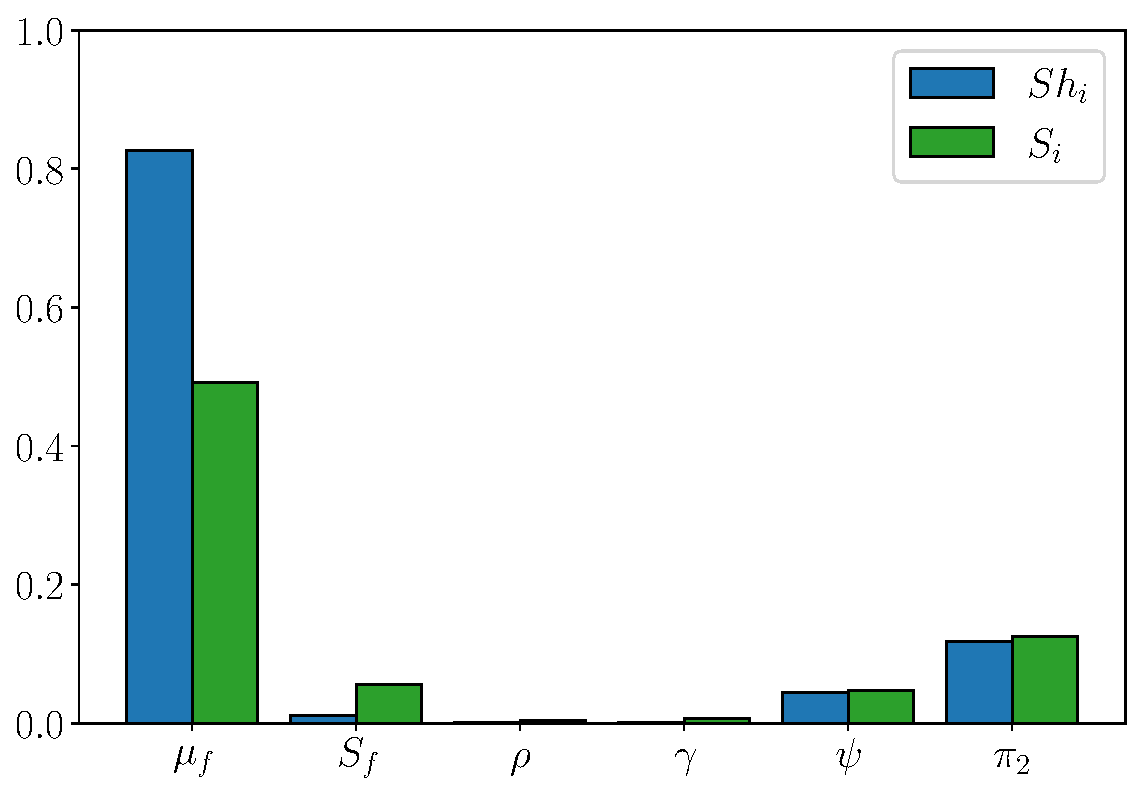
\includegraphics[width=\linewidth]{figures/scc_shapley_learning.pdf}\\[2pt]
{\scriptsize with learning}
\end{center}
\end{columns}

\vspace{0.2cm}
{\footnotesize Shapley values and first-order Sobol' indices for the SCC in 2020. The ranking is the deliverable: it says which of the deeply contested parameters the answer is actually sensitive to, and which of the arguments in the literature are, for this purpose, beside the point.}
\end{frame}

% --- Takeaways + hinge ---
\begin{frame}{UQ Takeaways, and the Turn to Part V}
\begin{itemize}\itemsep3pt
  \item SCC uncertainty is driven almost entirely by the prior belief about the \emphc{climate feedback factor} $\mu_{f,0}$ (an ECS of ${\approx}3.4$\,\textdegree C at the benchmark, and ${\approx}80\%$ of the Shapley mass read off the chart) and by the \textbf{damage curvature} $\pi_2$. Over the ranges considered, the discount rate, risk aversion and the EIS contribute \textbf{almost nothing}.
  \item That uncertainty \textbf{resolves in roughly a decade}, which itself changes optimal policy today.
  \item The whole analysis was post-processing: \emphc{the equilibrium was solved once}.
\end{itemize}

\vspace{0.15cm}
\begin{alertblock}{From describing to deciding}
Everything so far has been \emph{descriptive}: which parameters fit the data, which uncertainties matter. \emphc{Part V asks which policy is best}: same pipeline, same GP with active learning, but the operator becomes a \emphc{constrained} $\argmax$, with 40 cohort welfares as constraints.
\end{alertblock}
\end{frame}

% ============================================================================
% PART V: OPTIMAL CARBON TAX
% ============================================================================

\section{Design: The Optimal Carbon Tax}

\begin{frame}{}
\begin{center}
{\Huge \textcolor{uzhblue}{Part V}}\\[0.8em]
{\LARGE Design: The Optimal Carbon Tax}
\end{center}
\end{frame}

% --- The wall ---
\begin{frame}{The Design Problem}
\footnotesize
\begin{columns}[T]
\column{0.48\textwidth}
\textbf{Why this is hard economics}
\begin{itemize}\itemsep2pt
  \item Carbon pricing is the consensus instrument, but with \textbf{overlapping generations} a simple tax creates winners and losers.
  \item The losers are the \emph{currently alive}, and they vote. Optimal and politically dead is not a policy.
  \item So the object is a \textbf{constrained} optimum: maximize welfare \emph{subject to no cohort being made worse off}.
\end{itemize}

\column{0.48\textwidth}
\textbf{Why this is hard computation}
\begin{itemize}\itemsep2pt
  \item A 12-period stochastic OLG IAM with stochastic carbon intensity and a stochastic tipping point.
  \item Expected welfare at \emph{one} policy is $10{,}000$ forward simulations, about \emph{two seconds}. Cheap, until you notice the constrained search needs \emphc{millions} of queries, of the objective \emph{and} of 40 cohort-welfare surfaces.
  \item The Pareto constraint is on \emphc{40 cohort welfares}, not one aggregate.
\end{itemize}
\end{columns}

\vspace{0.3em}
\emphc{This is the wall.} Parts I to IV were built to get through it: pseudo-states so the equilibrium is solved once, a GP so the welfare surface is mapped from a few hundred points, and active learning so those points are well spent.

\vspace{0.15em}
{\scriptsize K\"ubler, Scheidegger \& Surbek (2026), in \texttt{../readings}.}
\end{frame}

% --- Policy coefficients as pseudo-states ---
\begin{frame}{Policy Coefficients as Pseudo-States}
\small
\begin{block}{The move, one more time}
The tax is a \emph{rule}, linear in cumulative emissions,
\[
\tau_t(E_t) = \vartheta_0 + \vartheta_E E_t ,
\]
with revenue recycled through a sharing rule. The coefficients $\pol$ are \emphc{embedded as pseudo-states in the DEQN}, as $\varrho$ was in Part II and $\str$ in Part IV.
\end{block}

\vspace{0.1cm}
\begin{columns}[T]
\column{0.5\textwidth}
\textbf{Surrogate 1: the equilibrium}
\begin{itemize}\itemsep1pt
  \item DEQN over the $d_x = 17$ state \emph{plus} the policy pseudo-states: $2$, $14$, then $\emphc{16}$ across the three scenarios, a \emphc{33-dimensional} solve at the top end
  \item Several hours from scratch, minutes warm-started
\end{itemize}
\column{0.48\textwidth}
\textbf{Surrogate 2: the welfare surface}
\begin{itemize}\itemsep1pt
  \item Maps $\pol \mapsto \E{\mathcal{W}(\pol)}$, plus one GP \emph{per cohort} for the constraints
  \item Built from surrogate 1, and it is what we optimize
\end{itemize}
\end{columns}

\vspace{0.04cm}
{\footnotesize \emphc{Cross-reference to this morning:} the pathology here is \emph{lazy learning}: low residual, nearly flat in $\pol$. Cure: anchors and distillation, Part VI of the DEQN deck.}
\end{frame}

% --- Welfare surrogate ---
\begin{frame}{The Welfare Surrogate: 500 Solves}
\small
\begin{columns}[T]
\column{0.315\textwidth}
\begin{block}{1. The mapping}
$\pol \longmapsto \E{\mathcal{W}(\pol)}$, a Monte Carlo mean of lifetime utilities.

\vspace{2pt}
\emphc{One training point $=$ 10{,}000 simulated paths.}
\end{block}
\column{0.315\textwidth}
\begin{block}{2. The design}
450 by \emph{uniform} sampling over the policy box (the DEQN's own design), then \emphc{50 by active learning}.

\vspace{2pt}
Total \emphc{500}, rising to 800 for the Pareto scenarios.
\end{block}
\column{0.315\textwidth}
\begin{block}{3. The model}
Squared exponential with automatic relevance determination.

\vspace{2pt}
\emphc{Leave-one-out error $3.2\times10^{-5}$}, against a stopping threshold of $10^{-4}$.
\end{block}
\end{columns}

\vspace{0.3cm}
{\footnotesize \textbf{Why ARD earns its keep:} one length scale per dimension makes the fitted kernel \emph{report} which policy coefficients the welfare surface responds to: a long length scale means that one barely matters. A free sensitivity analysis of the policy space, delivered with the fit.

\vspace{3pt}
\textbf{And note what 500 replaces.} Mapping the surface by brute force means a grid: even 4 points per axis is $4^{d}$ evaluations, each one 10{,}000 simulated paths. At $d = 2$ that is affordable; by $d = 16$ it is $4.3 \times 10^{9}$. The GP reconstructs the surface from a few hundred well-placed points either way.}
\end{frame}

% --- Three scenarios ---
\begin{frame}{Three Policy Scenarios}
\small
\begin{itemize}\setlength\itemsep{1.0em}
  \item \textbf{Scenario 1: unconstrained welfare maximization.}\\
  Linear tax on cumulative emissions, transfers fixed by an exogenous sharing rule.
  \vspace{-4pt}
  \[ \tau_t(E_t) = \vartheta_0 + \vartheta_E E_t \]
  \item \textbf{Scenario 2: Pareto-improving policy.}\\
  Same tax rule, but the \emphc{transfers are now optimized} subject to no cohort losing.
  \vspace{-4pt}
  \[ \tau_t(E_t) = \vartheta_0 + \vartheta_E E_t, \qquad \text{transfer shares} \in \pol \]
  \item \textbf{Scenario 3: more instruments.}\\
  Tax also on carbon intensity $\kappa_t$ and on proximity to the tipping point, with optimal transfers.
  \vspace{-4pt}
  \[ \tau_t = \vartheta_0 + \vartheta_E \tfrac{E_t}{E_0} + \underbrace{\vartheta_\kappa \tfrac{\kappa_t}{\kappa_0}}_{\text{intensity}} + \underbrace{\vartheta_{TP}(1 - \mathbb{D}_{TP})}_{\text{tipping risk}} \]
\end{itemize}
\end{frame}

% --- Scenario 1 surface ---
\begin{frame}{Scenario 1: The Welfare Surface}
\begin{columns}[c]
\column{0.55\textwidth}
\begin{center}
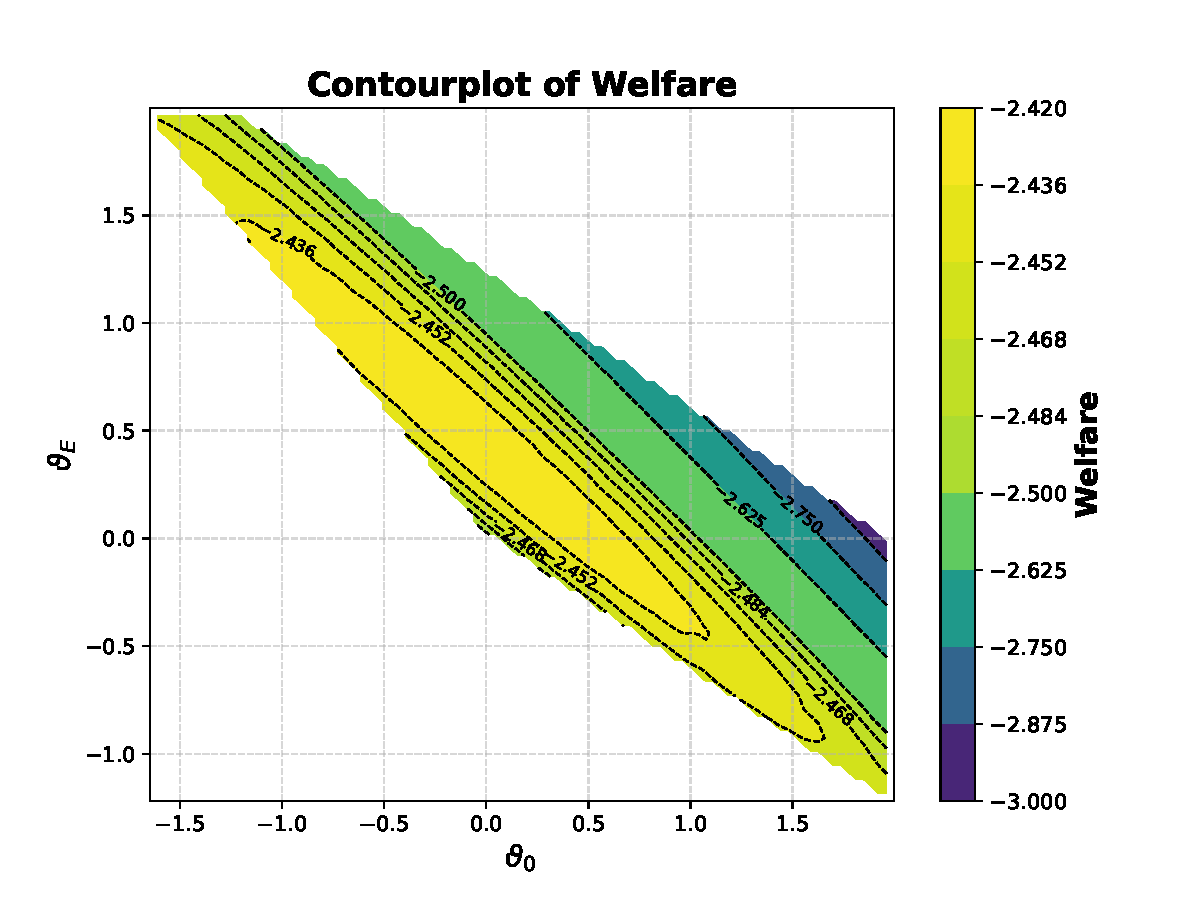
\includegraphics[width=\linewidth]{figures/contour_welfare_E.pdf}
\end{center}
\column{0.42\textwidth}
\small
\begin{itemize}\itemsep0.7em
  \item The GP posterior mean of social welfare over the tax intercept $\vartheta_0$ and slope $\vartheta_E$.
  \item The optimum is the interior peak. Finding it is now a \emphc{constrained $\argmax$ on a smooth surface}, the same operator as Part II's $\argmin$, opposite sign of intent.
  \item Constraints keep the implied tax rate inside $[0, \bar\tau]$ at both ends of the horizon.
  \item \emphc{The surface is a picture, not an optimizer's report}, exactly the advantage a cheap surrogate buys.
\end{itemize}
\end{columns}
\end{frame}

% --- Scenario 1 price ---
\begin{frame}{Scenario 1: The Aggregate Gain, and Who Pays for It}
\begin{columns}[c]
\column{0.55\textwidth}
\begin{center}
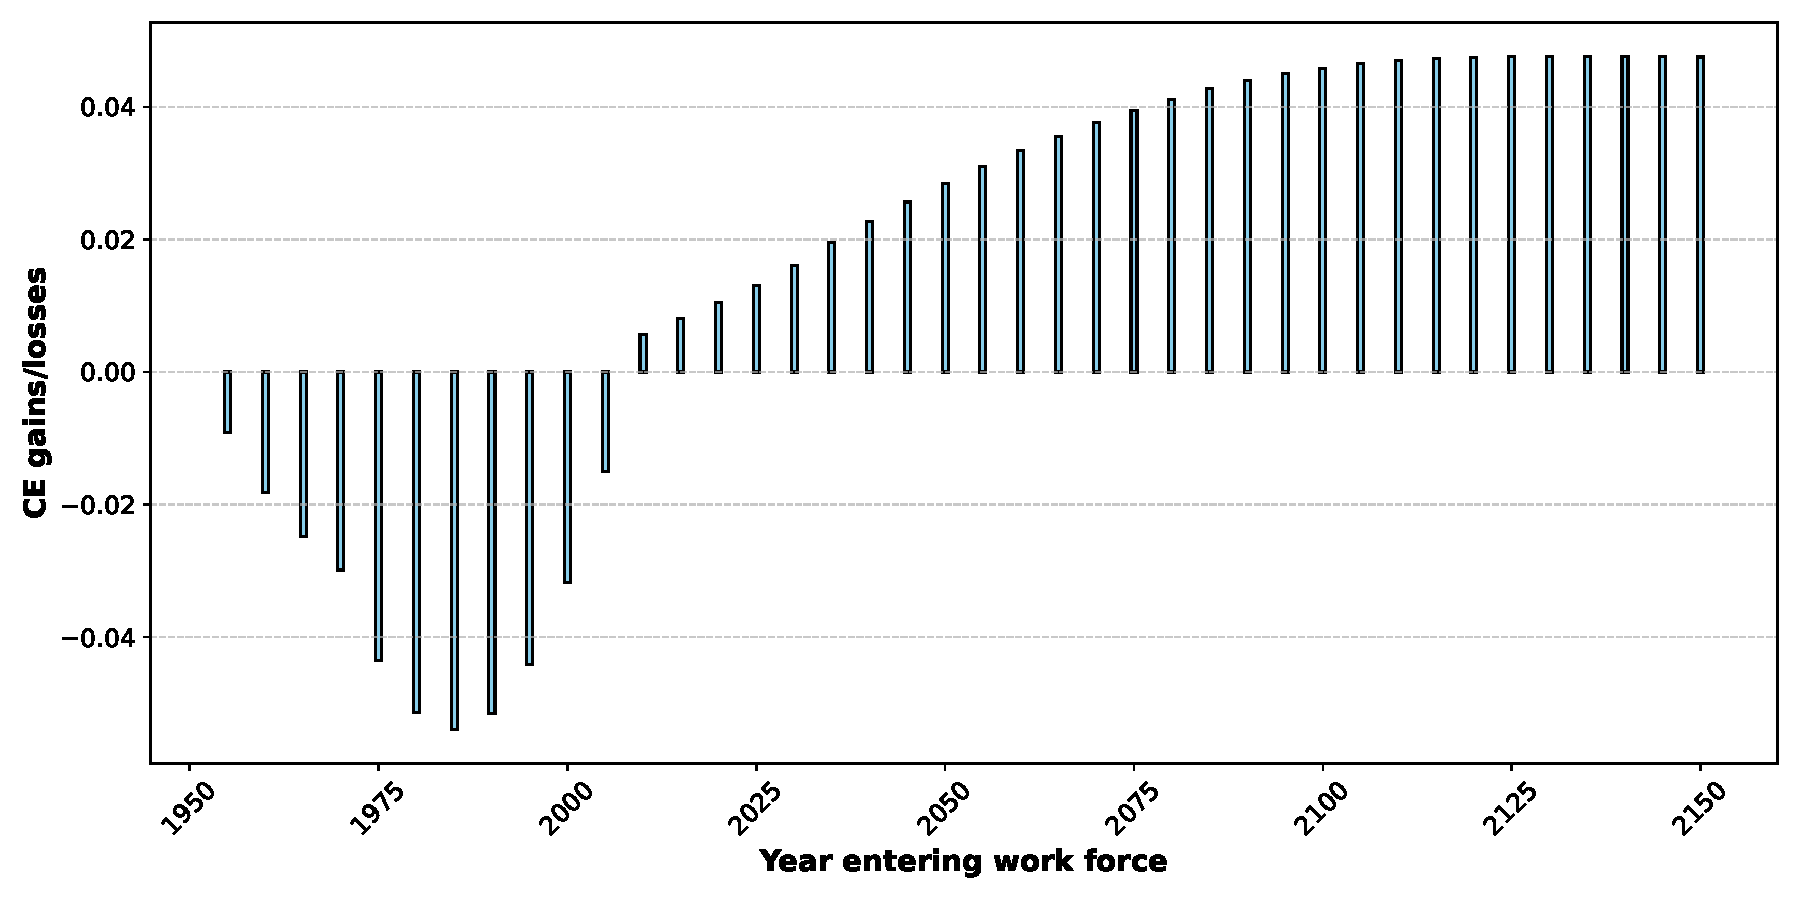
\includegraphics[width=\linewidth]{figures/lin_S_10trans_unif_welfares.pdf}
\end{center}
\column{0.42\textwidth}
\small
\begin{itemize}\itemsep0.7em
  \item \textbf{Aggregate welfare} rises by \emphc{1.6\%} in consumption-equivalent terms.
  \item Cohorts entering the workforce from about 2100 on gain up to \emphc{4.8\%}.
  \item \textcolor{harvardcrimson}{\ding{55}~\textbf{But:}} every cohort that entered before ${\approx}2007$ (everyone working today) loses, by up to \emphc{5\%}.
  \item \textbf{Conclusion:} without transfers, the welfare-maximizing carbon tax is \emphc{politically dead on arrival}, and no amount of aggregate-welfare arithmetic changes that.
\end{itemize}
\end{columns}
\end{frame}

% --- Scenario 2 ---
\begin{frame}{Scenario 2: Buying Consensus with Transfers}
\begin{columns}[c]
\column{0.55\textwidth}
\begin{center}
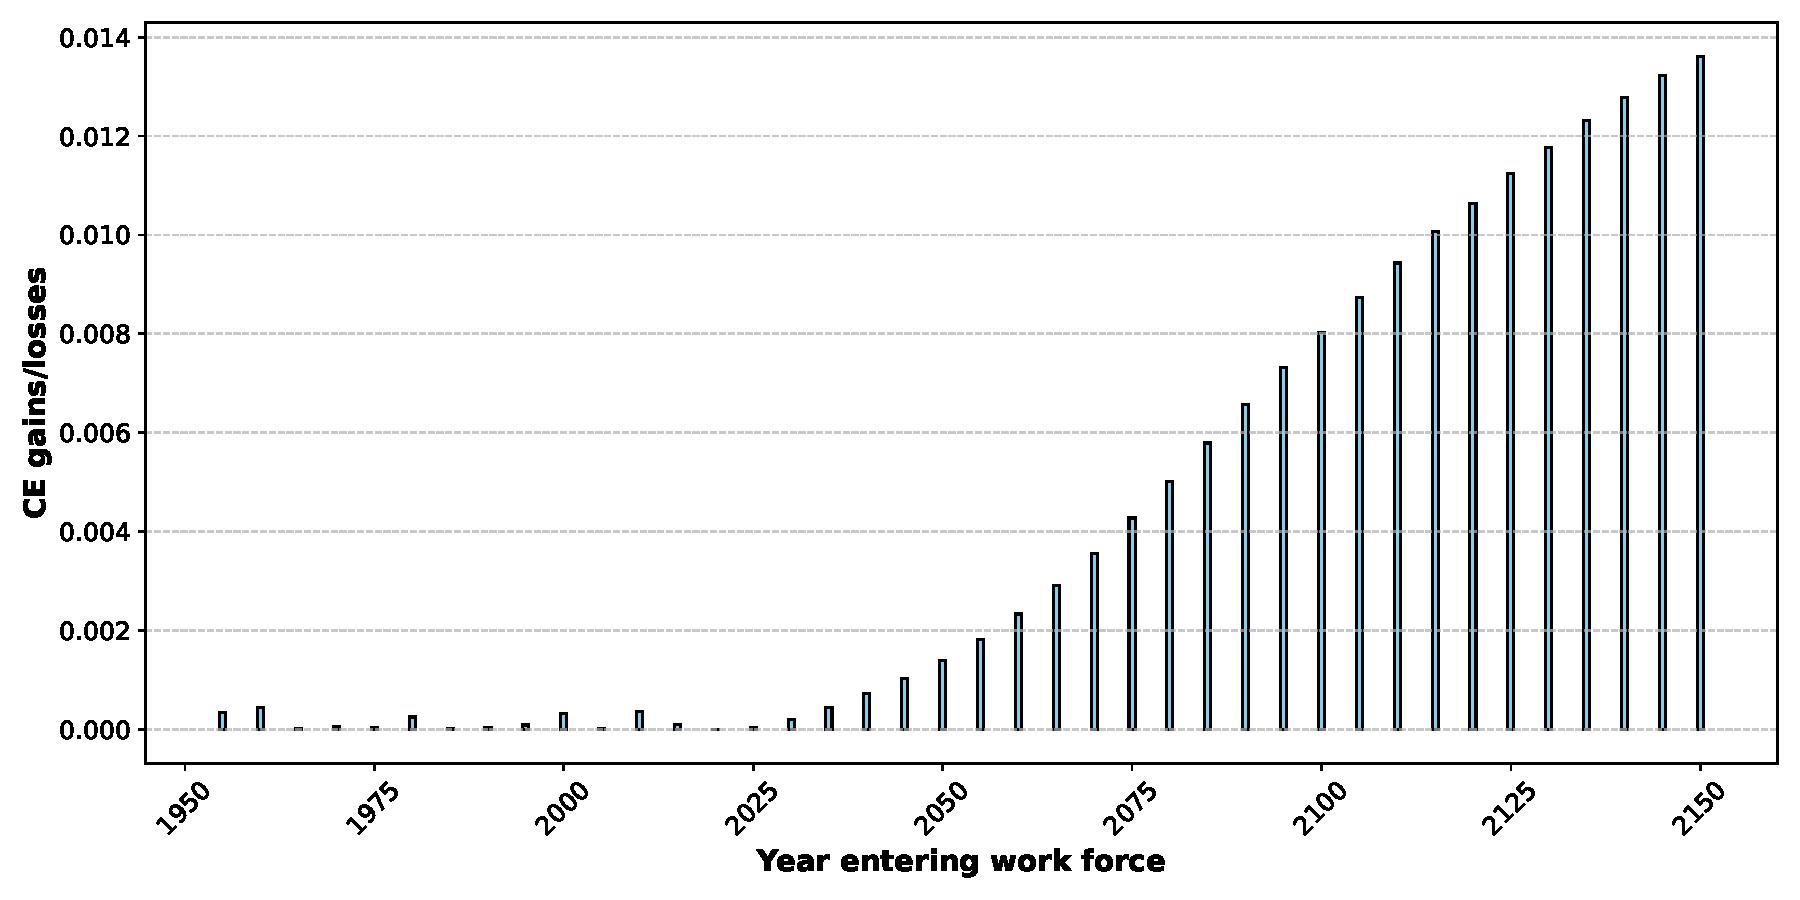
\includegraphics[width=\linewidth]{figures/welfare_gains_lin_S_trans.pdf}
\end{center}
\column{0.42\textwidth}
\small
\begin{itemize}\itemsep0.6em
  \item \textbf{The constraint:} transfers are optimized so that initial generations, and those born over the next decade, stay at \emphc{business-as-usual welfare}: zero loss, by construction.
  \item \textbf{Future gains:} flat at zero for cohorts alive today, then rising steadily to \emphc{${\approx}1.4\%$} by 2150.
  \item \textbf{The price of consensus:} smaller than the unconstrained 4.8\%, but \emphc{no generation loses}.
  \item \textbf{Aggregate:} \emphc{0.42\%}, about a quarter of the unconstrained gain.
\end{itemize}
\end{columns}
\end{frame}

% --- Scenario 2 temperature ---
\begin{frame}{What the Policy Actually Does}
\begin{columns}[c]
\column{0.5\textwidth}
\begin{center}
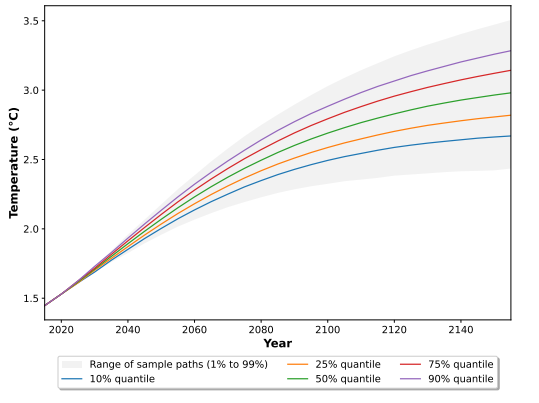
\includegraphics[width=\linewidth]{figures/Temp_case2.png}
\end{center}
\column{0.47\textwidth}
\small
\begin{itemize}\itemsep0.45em
  \item \textbf{Mean warming} settles just below \emphc{3\,\textdegree C}, \emph{higher} than unconstrained.
  \item \textbf{The 99th percentile never exceeds 3.5\,\textdegree C}, against a much fatter tail under business as usual.
  \item It buys not a lower average but a \emphc{truncated tail}.
  \item \textcolor{uzhblue}{\textbf{Reading:}} the tax works as \emphc{disaster insurance}, not aggressive mitigation.
  \item {\footnotesize \emph{Caveat:} the tipping threshold is confined to $[2.5,3.5]$\,\textdegree C by construction, so this says the policy pushes the distribution \emph{off} the upper barrier.}
\end{itemize}
\end{columns}
\end{frame}

% --- Scenario 3 ---
\begin{frame}{Scenario 3: Does Policy Complexity Pay?}
\small
Adding instruments means adding pseudo-states: the policy space grows from $d_{\pol} = 14$ to $\emphc{16}$ (4 tax parameters plus 12 transfer shares). At the optimum,
\[
\{\vartheta_0,\; \vartheta_E,\; \vartheta_\kappa,\; \vartheta_{TP}\} = \{-0.237,\; 0.203,\; 0.037,\; 0.012\}.
\]

\begin{center}
\begin{tabular}{lcc}
\toprule
\textbf{Policy specification} & \textbf{Instruments} & \textbf{Aggregate welfare gain} \\
\midrule
Linear in cumulative emissions $E_t$ & 2 & \textbf{0.42\%} \\
Linear in $E_t$, $\kappa_t$, $TP_t$ & 4 & \textbf{0.45\%} \\
\bottomrule
\end{tabular}
\end{center}

\vspace{0.25cm}
\begin{alertblock}{Diminishing returns}
A simple, well-designed tax on cumulative emissions captures \emphc{93\%} of the achievable welfare gain. The two extra instruments (taxing carbon intensity and proximity to the tipping point) buy almost nothing \emph{once intergenerational participation constraints are imposed}.

\vspace{2pt}
Note the qualifier. It is the Pareto constraint, not the physics, that flattens the return to complexity.
\end{alertblock}
\end{frame}

% --- Cost of feasibility ---
\begin{frame}{The Cost of Political Feasibility}
\small
\begin{columns}[T]
\column{0.48\textwidth}
\textbf{1. Welfare maximizing} (unconstrained)
\begin{itemize}\itemsep2pt
  \item Aggressive early mitigation
  \item Warming stabilizes near \emphc{2.7\,\textdegree C}
  \item \textcolor{harvardcrimson}{\ding{55}~Current generations lose up to 5\%}
  \item Aggregate gain 1.6\%
\end{itemize}
\column{0.48\textwidth}
\textbf{2. Pareto improving} (constrained)
\begin{itemize}\itemsep2pt
  \item Slower initial mitigation path
  \item Warming stabilizes near \emphc{3.0\,\textdegree C}
  \item \textcolor{darkgreen}{\ding{51}~No generation loses}
  \item Aggregate gain 0.42\%, tail cut
\end{itemize}
\end{columns}

\vspace{0.3cm}
\begin{alertblock}{The trade-off, stated plainly}
Securing political support requires delaying some mitigation, costing about \emphc{$+0.3$\,\textdegree C} in mean warming. In exchange it eliminates the extreme-damage scenarios, insuring future generations against disasters rather than shaving the average.

\vspace{3pt}
\emphc{None of this was visible before the surrogate.} The comparison requires optimizing a 16-dimensional constrained problem whose objective needs 10{,}000 simulations per query, which is to say, it requires everything in Parts I to IV.
\end{alertblock}
\end{frame}

% ============================================================================
% PART VI: SYNTHESIS
% ============================================================================

\section{Synthesis and Hands-On}

\begin{frame}{}
\begin{center}
{\Huge \textcolor{uzhblue}{Part VI}}\\[0.8em]
{\LARGE Synthesis and Hands-On}
\end{center}
\end{frame}

% --- One surrogate three questions ---
\begin{frame}{One Surrogate, Three Questions}
\footnotesize
\begin{center}
\setlength{\tabcolsep}{3pt}
\begin{tabular}{>{\raggedright\arraybackslash}p{0.155\textwidth}>{\raggedright\arraybackslash}p{0.235\textwidth}>{\raggedright\arraybackslash}p{0.235\textwidth}>{\raggedright\arraybackslash}p{0.235\textwidth}}
\toprule
 & \textbf{Part II: estimate} & \textbf{Part IV: quantify} & \textbf{Part V: design} \\
\midrule
Model & Brock--Mirman & stochastic IAM with Bayesian learning about the climate sensitivity & stochastic OLG IAM with tipping risk \\
Surrogate 1 inputs & $(z, K, \beta, \varrho)$ & climate-economy states plus uncertain $\str$ & OLG state plus 16 policy pseudo-states \\
QoI & moments $m_1$ to $m_3$ & $\mathrm{SCC}(\str)$ & 40 cohort welfares \\
Surrogate 2 & none needed & GP $+$ active learning & 40 GPs $+$ active learning \\
Operator & $\argmin$ under common random numbers & global sensitivity: univariate effects, Sobol', Shapley & constrained $\argmax$ \\
Output & an interior estimate & an importance ranking & a Pareto-improving tax \\
Headline & a flat direction is the moments \emph{or} the surrogate & climate sensitivity and damages drive the SCC & 0.42\% gain, and the tail is cut \\
\bottomrule
\end{tabular}
\end{center}
\end{frame}

% --- Toolbox ---
\begin{frame}{The Toolbox: When to Use What}
\begin{center}
\footnotesize
\begin{tabular}{l l l}
\toprule
\textbf{Method} & \textbf{Use when} & \textbf{Watch out for} \\
\midrule
Polynomials, splines & $d \le 3$, smooth, cheap labels & no kinks, no irregular domains \\
Sparse grids & $d \lesssim 20$, local features matter & tensor structure, hypercube domain \\
\emphc{Gaussian process} & \emphc{labels expensive}, $d \lesssim 10$ & $\mathcal{O}(N^3)$; the kernel \emph{is} the model \\
\emphc{Deep network} & \emphc{labels cheap}, $d$ large & no uncertainty; architecture search \\
GP $+$ active learning & every evaluation is precious & sequential, so hard to parallelize \\
\bottomrule
\end{tabular}
\end{center}

\vspace{0.2cm}
\begin{block}{A decision procedure, in order}
\small
\begin{enumerate}\itemsep1pt
  \item \textbf{Price one label.} Seconds, or hours? That number decides more than anything else here.
  \item \textbf{Count the dimensions} \emph{after} promoting parameters to pseudo-states, not before.
  \item \textbf{Ask whether you need an error bar.} If a decision rides on the surrogate, you do.
  \item \textbf{Layer them} when model and quantity of interest have different cost profiles, the common case.
\end{enumerate}
\end{block}
\end{frame}

% --- Practical guidance ---
\begin{frame}{Practical Guidance}
\small
\begin{itemize}\itemsep4pt
  \item \textbf{Train once, then simulate for free.} Surrogate 1 costs hours from scratch and minutes warm-started. Every downstream question is then a forward pass. Budget accordingly: the expensive part is the design, not the training.
  \item \textbf{Validate \emph{in the parameter direction}, not on average.} A surrogate with excellent mean error can still be nearly flat in $\str$: low residual, wrong policy. This is \emphc{lazy learning}; the cure (anchors and distillation) is Part VI of this morning's deck. \emphc{Do not skip this check}; it is the most common way a surrogate study goes quietly wrong.
  \item \textbf{Report leave-one-out error, not training error}, and report the \emphc{maximum} over the parameter box, not the mean. The maximum is what bounds the bias in $\str^\star$.
  \item \textbf{Use common random numbers whenever you sweep a parameter.} Without them you are optimizing simulation noise, in estimation \emph{and} in policy design.
  \item \textbf{When one quantity-of-interest evaluation is expensive, add the second surrogate.} Expected welfare at one policy took 10{,}000 Monte Carlo paths; the GP layer cut the whole study to 500 simulations at leave-one-out error $3.2\times10^{-5}$.
\end{itemize}
\end{frame}

% --- Hands-on ---
\begin{frame}{Hands-On: What to Run}
\small
Notebooks in \texttt{../code/03\_deep\_surrogates}: PyTorch $+$ scikit-learn, CPU-only, self-contained. \texttt{03\_01} and \texttt{03\_02} ship on \texttt{RUN\_MODE = "smoke"}; raise it once a run works.

\vspace{0.15cm}
\begin{itemize}\itemsep4pt
  \item \textbf{A deep surrogate, end to end} \emph{(${\approx}3.5$ min)}. Black--Scholes over $(S, K, T, \sigma, r)$, then implied-vol inversion by root-finding \emph{and} by gradient descent. \emphc{Read its timing table:} on this toy the surrogate \emph{loses} to numpy: the ``price one label first'' rule biting. \hfill{\footnotesize\texttt{03\_01}}
  \item \textbf{GP regression and active learning} \emph{(${\approx}30$ s)}. A GP from scratch in numpy, checked against \texttt{sklearn}; then the BAL loop and its budget sweep. \hfill{\footnotesize\texttt{03\_02}}
  \item \textbf{Estimating $\varrho$ by SMM} \emph{(${\approx}10$ s)}. Train with $\varrho$ as a pseudo-state, simulate under common random numbers, recover the parameter. \hfill{\footnotesize\texttt{03\_03}}
  \item \textbf{The identification ridge} \emph{(${\approx}10$ s)}. Free $\beta$ as well, watch the valley appear, and read the moment Jacobian's singular values. \hfill{\footnotesize\texttt{03\_04}}
\end{itemize}

\vspace{0.15cm}
{\footnotesize \textbf{If you only run one:} \texttt{03\_02}. It builds a GP from scratch, and its budget sweep is the measurement behind the honest version of the active-learning claim.}
\end{frame}

% --- Closing ---
\begin{frame}{}
\begin{columns}[c]
\column{0.42\textwidth}
\begin{center}
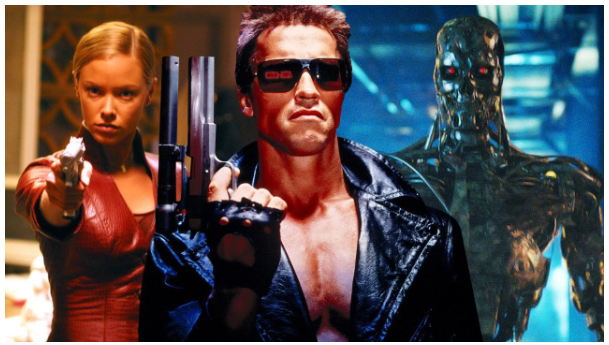
\includegraphics[width=0.8\linewidth]{figures/quest.png}
\end{center}
\column{0.55\textwidth}
{\LARGE \textcolor{uzhblue}{Questions?}}

\vspace{0.5cm}
{\small
\textbf{Simon Scheidegger}\\
HEC, University of Lausanne\\[4pt]
\href{mailto:simon.scheidegger@unil.ch}{simon.scheidegger@unil.ch}~~$\cdot$~~\href{https://sischei.github.io}{sischei.github.io}
}

\vspace{0.5cm}
{\footnotesize
\textbf{Next up, 15:30 -- 17:00:} \emph{Solving heterogeneous agent models with DeepHAM and structural reinforcement learning} (Yang), where the model whose parameters we just estimated becomes one with a full cross-sectional distribution.
}

\vspace{0.4cm}
{\footnotesize
\textbf{Materials:}~\href{https://github.com/sischei/summer-school-AI-for-economics-and-finance-2026}{github.com/sischei/summer-school-AI-\ldots-2026}\\
\textbf{Cloud:}~\href{https://nuvolos.cloud}{nuvolos.cloud}
}
\end{columns}
\end{frame}

\end{document}
